
\chapter{Irradiation of cardiac target volumes in porcine data}
\label{chapter:porcine}
\minitoc

The presented results of planning studies for a non-invasive ablation of cardiac target sites in human data need to be experimentally 
validated. This will be carried out at GSI in 2014, in collaboration with HIT and University Hospital Heidelberg as well as Mayo Clinic 
(Rochester, Minnesota, USA). Porcine models will be used and the results will be compared to findings with photon irradiation, both from 
literature \cite{Sha10, Bla13}, as well as from studies currently performed at Mayo Clinic. For the feasibility study different cardiac 
target sites are conceivable: PV isolation, ablation of the CTI as well as the AV node. In a first iteration of the experiments, only the AV 
node of the pigs will be irradiated, both at Mayo Clinic with photons and at GSI with carbon ions. The experiments are planned to enable a 
direct comparison between particle therapy and photon irradiation, so that many of the treatment settings are kept constant inbetween the two 
centers. Also in pigs, cardiac target sites move due to respiration as well as heartbeat, causing potential interplay effects 
which threaten the treatment oucome. While the breathing motion of the pigs is planned to be compensated with breath hold, controlled 
by a respirator, the influence of heartbeat motion needs to be studied in more detail. The resulting motion amplitude and direction will be 
studied and rescanning as motion mitigation technique will be presented.

\section{Material and methods}
As in the previous chapter, the input data and treatment planning parameters will be given before stating all performed studies. 
Finally, the analysis procedure will be described.  

\subsection{Treatment planning input data}
In order to assess the motion of the potential cardiac target sites (PV, CTI and AV node) in pigs under influence of heartbeat motion, 
ECG gated 4DCTs were studied. Four porcine data sets were recorded at Mayo Clinic (Rochester, Minnesota, USA) under anesthesia and respiration.  
The CT scans were acquired on a Definition Dual Source CT scanner (Siemens). The 4DCT data set consisted of twenty temporal equally distributed 
cardiac motion phases, the reference phase zero started at the R-peak of the QRS-complex (see chapter \ref{chapter:intro}, section \ref{HCS}). 
Native CT scans were recorded. In order to distinguish structures within the heart, contrast enhanced CT scans were also aquired directly 
after the native scans. The radiopaque material was administered intravenously (100 mL contrast media at a rate of 4 mL/sec) and the CT scans 
were acquired 30 seconds after injection.
Segmentation of the target volumes as well as the OARs (esophagus, trachea, aorta and cardiac structures) were carried out by a collaborating 
cardiologist at Mayo Clinic with Eclipse\texttrademark (Varian Medical Systems) on the reference phase. The volumes of the contours for the 
different ablation sites are presented for each pig in table \ref{tab:volume:mayo:porcine}. The location of these sites are visualized in 
figure \ref{pig1_targets} exemplarily for pig 1. Contrary to humans pigs have only one PV pair, distinguished inbetween inferior PV (IPV) and 
superior PV (SPV). The contour for the PV encircles both of these structures. 

% \vspace*{-0.6cm}

\begin{table}[htbp]
% \footnotesize
  \centering
  \caption{Target volume for the different cardiac target sites for all investigated pigs.}
  \begin{tabular}{|c|c|c|c|}
    \hline\hline
    pig no\rule{0pt}{2.6ex}\rule[-1.2ex]{0pt}{0pt} & PVs [cm$^{3}$] & CTI [cm$^{3}$] & AV [cm$^{3}$]\\
    \hline
    1 & 0.72 & 0.20 & 0.08 \\
    2 & 1.01 & 0.13 & 0.05 \\
    3 & 1.09 & 0.24 & 0.06 \\
    4 & 1.03 & 0.31 & 0.02 \\
    \hline\hline
  \end{tabular}
  \label{tab:volume:mayo:porcine}
\end{table}

\newpage

 \begin{figure}[H]
 \begin{center}
\subfigure[PVs and AV node]{
 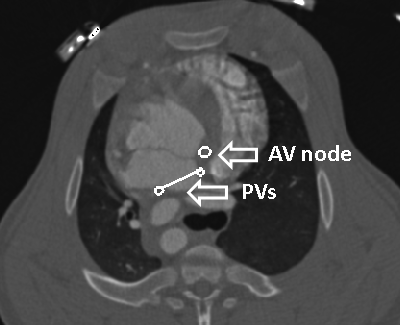
\includegraphics[scale=0.75]{./teile/results_porcine/L829_PVsandAV_2.png}
 }
\subfigure[PVs and CTI]{
 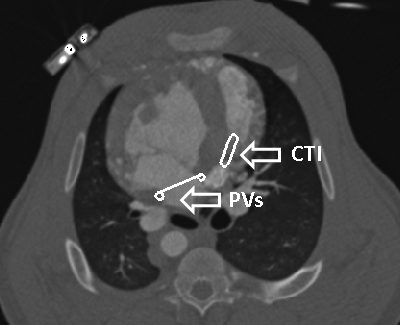
\includegraphics[scale=0.75]{./teile/results_porcine/L829_PVsandCTI_2.png}
 }
\caption{Cardiac target volumes (PV, CTI and AV node) in pig 1. }
\label{pig1_targets}
 \end{center}
\end{figure}

\vspace*{-0.7cm}

Also for these data sets, non-rigid image registration of the nineteen motion phase on the reference phase has been performed with Plastimatch 
\cite{Sharp07, Shack10}. The first step of the B-Spline registration was carried out with 50 maximal iterations and an isotropic 
spacing of 4mm, while the second step had maximal 100 iterations with a grid spacing of 1mm. For the contrast enhanced CT scans the 
regularization was chosen to be $\lambda$=0.005, while for the native CT scans $\lambda$=0.0001 was chosen . 
The quality of registration was also here validated with visualization techniques (false color images \cite{Bro07}, checker board images 
\cite{Bro07} and aqualitative check of the vector field regularization) between motion phase 3 and the reference phase 0 and motion 
phase 18 and the reference phase.  

\subsection{Treatment planning parameters}

All treatment plans were generated on contrast-enhanced CT scans (see section \ref{subsec:motion:pigs}) without motion (3D, static) as well as 
with motion (4D).  For informations on the dose optimization process, the used raster spacing, dose 
algorithm and GSI beam applications the reader should be referred to \ref{human:tpp}.\newline
\newline
Besides the original volume of the CTV, a safety margin has been added to the volumes of the treatment planning study. In agreement with the 
Mayo Clinic radiooncology an isotropic safety margins of 5mm has been chosen, which will also be applied in the irradiation with photons. 
The ITV volumes\cite{Gra12}, which were obtained from all twenty motion phases and were used as the final target, were generated from the 
original CTV contour as well as from the CTV with margin, so that potential range variations were considered in the margins.
\newpage
All treatment plans were calculated as single field uniform dose (SFUD) deliveries, applying a physical dose of 25Gy in one fraction. The minimum particle number per beam spot was set to 75,000.
The dose was applied from two different beam channel directions. With the fixed horizontal beam line available at GSI the beam positions 
were chosen as two lateral fields with couch angles of -90$^{\circ}$ and 90$^{\circ}$. With these opposing fields the treatment should be 
more robust against potential uncertainties like range differences. Due to the GSI specific beam output, the particles are applied at an 
angle of -2.203$^{\circ}$, which was integrated in the treatment plans as a gantry angle.\newline
\newline
As the reconstruction of the 4DCTs was based on the time scale a phase-based motion state detection was employed. 
In order to consider possible divergence in the heartbeat motion pattern of the pigs, different motion periods (0.7s and 0.5s) as well as 
different starting phases (0$^{\circ}$ and 90$^{\circ}$) were used. The fast motion periods were chosen according to the  
heartbeat rate of the pigs, between 110 and 120 beats per minute.


\subsection{Treatment planning studies}

On the basis of 3D treatment plans on the AV node the dose to nearby OARs were studied (see table \ref{tab:RTOG:pig}). 
These were carried out on the CTV of all four pig data sets. Furthermore 3D (static) treatment plans were produced as reference values to the 
4D cases. 4D plans were distinguished between an underlying motion without any compensation, resulting in interplay patterns \cite{Phi92, Ber08}, 
and with the application of rescanning \cite{Phi92} as motion mitigation technique. For rescanning three different rescan 
numbers (5, 10 and 15) were compared.
Static, interplay as well as rescanning treatment plans for all pigs where carried out with the two stated beam entry channels,
a safety margin of 5mm, the stated treatment planning parameters and the four stated motion trajectories. 
All treatment planning studies were carried out on contrast enhanced CT scans due to the lack of contrast on native CT scans (see section 
\ref{subsec:motion:pigs}). 


\subsection{Analysis}

The dose deposition in the OAR as well as dose homogeneity in the target volume were studied. The dose deposition in the OARs 
(esophagus, trachea, aorta and the whole heart) were compared to dose-volume restriction stated in RTOG study protocols 
(see table \ref{tab:RTOG:pig}) \cite{RTOG0631, RTOG0915} (see chapter \ref{chapter:human}, section \ref{human:dose-volumeOar}). 
As further OAR cardiac substructures (ventricles and coronary arteries) were studied. Here the mean dose into the structures as well as the 
maximum point dose and the maximal irradiated volume (V$_{>0}$) were analyzed. Since the values were not normally distributed, the 
median (50th percentile) as well as the 75th percentile were calculated over all pigs. 
Motion-volume-histograms (MVHs) \cite{Ric13} were generated to display the relative displacement of every 
voxel of the investigated volume to the reference phase in all three motion directions. With these values the resulting motion of the cardiac 
target sites due to heartbeat could be assessed. In particular, the motion assessable from the native CT scans were compared with the contrast 
enhanced motion information. For comparison the resulting DVHs from the different techniques were studied. The V95 (measure of dose 
coverage), V107 (over dosage) and D5-D95 (dose homogeneity) to the CTVs were assessed. Futhermore the median and percentile values 
(25th and 75th) of these parameters over all studied motion patterns and patient cases were generated. In one case a one-way ANOVA was carried out 
and the proportion of variance explained $r^{2}$ is reported with the corresponding p-value ($p$<0.0001). 

% \vspace*{-0.5cm}

\begin{table}[H]
  \centering
%   \footnotesize
  \caption{Dose-volume limits for OAR.}
  \begin{tabular}{|c|c|c|c|}
    \hline\hline
    OAR & Volume [cc] & Dose [Gy] & endpoint \\
    \hline
    Aorta / great vessels & 10 & 31 & Aneurysm \\
    Esophagus & 5 & 11.9 &  Stenosis / fistula \\
    Heart & 15 & 16 & Pericarditis \\
    Trachea & 4 & 10.5 & Stenosis / fistula \\
    \hline\hline
  \end{tabular}
  \label{tab:RTOG:pig}
\end{table}


\section{Results}

In the following the results of the motion assessment due to heartbeat will be shown. Afterwards the dose to OAR when irradiating the AV node 
will be presented in detail. For the treatment planning study different dose analysis parameters will be presented and compared for different 
cases (static, interplay and rescanning). 

\subsection{Motion directions and magnitude}
\label{subsec:motion:pigs}
Treatment planning for particle therapy is carried out on native CT scans, as the Hounsfield units (HU) give information on the electron 
density of the structures and hence enable a calculation of the needed particle range. 
In native CTs, however, the contrast between the cardiac muscle and blood is low.  
A comparison between motion assessments of the cardiac target volumes 
in native and contrast-enhanced CT scans will be presented for one porcine data set. Afterwards the motion of all target volumes (PVs, CTI and 
AV node) will be shown for all pigs. 

\subsubsection*{Motion of cardiac target volumes in contrast enhanced versus native CT scans}
Only one of the four porcine data sets (pig 3) offered identical depicted anatomy between native and contrast enhanced data sets. For all 
other data sets the pig was moved inbetween the CT acquisitions. For a fair comparison this data set was hence analyzed. 
Using the resulting deformation maps from deformable image registration the motion of the ablation sites of PVs, CTI and AV node were assessed 
in both scans of pig 3. Motion volume histograms (MVHs) \cite{Ric13} displaying the relative displacement of every voxel of the investigated 
volume to the reference phase in all three motion directions were generated. The mean and standard deviation of these displacement values in 
each motion phase are plotted for all motion directions in figures \ref{motion_hb_pv_contrast_native} - \ref{motion_hb_av_contrast_native}.
It can be seen that the motion from the contrast enhanced CT is much larger than from the native CTs. While the mean absolute 
displacement in the native CT is smaller than 1mm in case of PVs and AV node and smaller than 1.5mm in case of CTI, the contrast CT enables a 
motion assessment which yields a mean absolute displacement of larger than 2mm in all studied target volumes (see table \ref{tab:motion_native_vs_contrast}). 
The difference is especially large in the AV node. The maximal observable displacement for this structure in case of the native CT scan is 
(0.2 $\pm$ 0.1)mm (MP 12), while with the contrast enhanced CT an absolute displacement of (2.5 $\pm$ 0.4)mm is 
assessable in this motion phase and the maximal absolute displacement is found to be (4.4 $\pm$ 0.1)mm (MP 5) (see Appendix \ref{app:pigs:mmt}). 
It can thus be concluded that contrast enhanced CTs are needed in order to fully assess the motion of cardiac target volumes in pigs. 
Since range deviations of contrast enhanced CT are in the order of 2.5\% compared to native CTs \cite{Wer04} and none of the treatment plans 
were applied in experiments, we decided to perform all subsequently presented calculations on contrast enhanced CTs. This allows to incorporate 
the larger motion amplitudes into the studies on influence of intrafractional motion. 

% % \newpage
% 
\vspace*{1cm}

\begin{table}[H]
  \centering
  \small
  \caption{Mean displacement of cardiac taget volumes in pig 3 over all motion phases.}
  \begin{tabular}{|c|c|c|c|c|c|}
    \hline\hline
    & Target & ABS [mm] & SI [mm] & AP [mm] & LR [mm] \\
    \hline\hline
    & PVs & 1.7 $\pm$ 0.8 & -0.2 $\pm$ 0.6 & 0.7 $\pm$ 0.9 & 0.1 $\pm$ 0.8 \\
    contrast CT & CTI & 1.6 $\pm$ 0.6 & 0.4 $\pm$ 0.5 & 0.7 $\pm$ 0.7 & 0.2 $\pm$ 0.6 \\
    & AV &  2.8 $\pm$ 0.4 & 0.0 $\pm$ 0.3 & 2.0 $\pm$ 0.3 & -1.4 $\pm$ 0.6 \\
    \hline
%     & Target & ABS [mm] & SI [mm] & AP [mm] & LR [mm] \\
%    \hline
    & PVs & 0.9 $\pm$ 0.4 & 0.0 $\pm$ 0.4 & 0.1 $\pm$ 0.5 & -0.1 $\pm$ 0.5 \\
    native CT & CTI & 1.1 $\pm$ 0.5 & -0.1 $\pm$ 0.6 & 0.6 $\pm$ 0.5 & -0.1 $\pm$ 0.5 \\
    & AV & 0.1 $\pm$ 0.1 & 0.1 $\pm$ 0.1 & 0.0 $\pm$ 0.1 & 0.0 $\pm$ 0.1 \\
    \hline\hline
  \end{tabular}
  \label{tab:motion_native_vs_contrast}
\end{table}

% % \vspace*{0.8cm}
% \vspace*{-0.5cm}

\newpage

\begin{figure}[H]
\begin{center}
 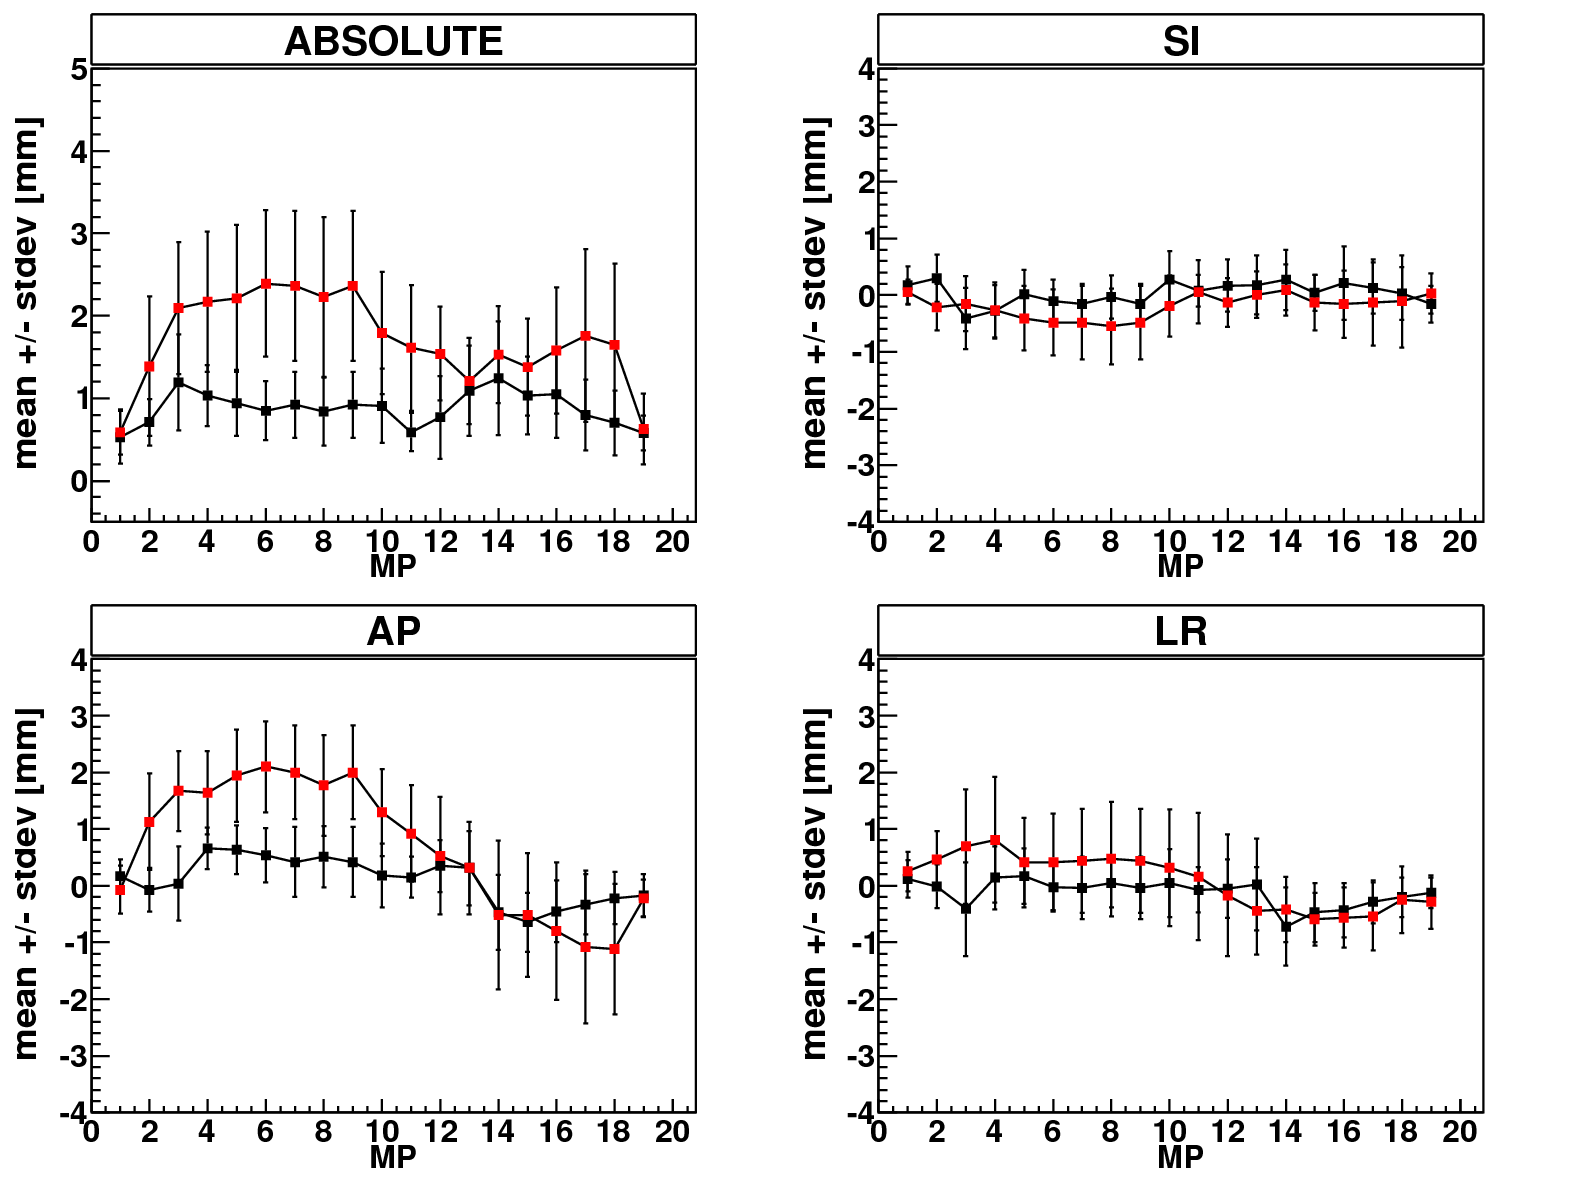
\includegraphics[scale=0.22]{./teile/results_porcine/Mayo_IPV_HB_NATIV_VS_CONTRAST.png}
\caption{PV: mean motion amplitude and standard deviation in each motion phase (MP) of the heartbeat relative to the reference phase. The 
displacement is shown for the three studied motion directions (SI: superior-inferior, AP: anterior-posterior, LR: left-right) and the absolute 
(ABS) displacment. Comparison between native CT data (black) and contrast CT (red) for Pig 3.}
\label{motion_hb_pv_contrast_native}
\end{center}
\end{figure}

\vspace*{-0.8cm}

\begin{figure}[H]
\begin{center}
 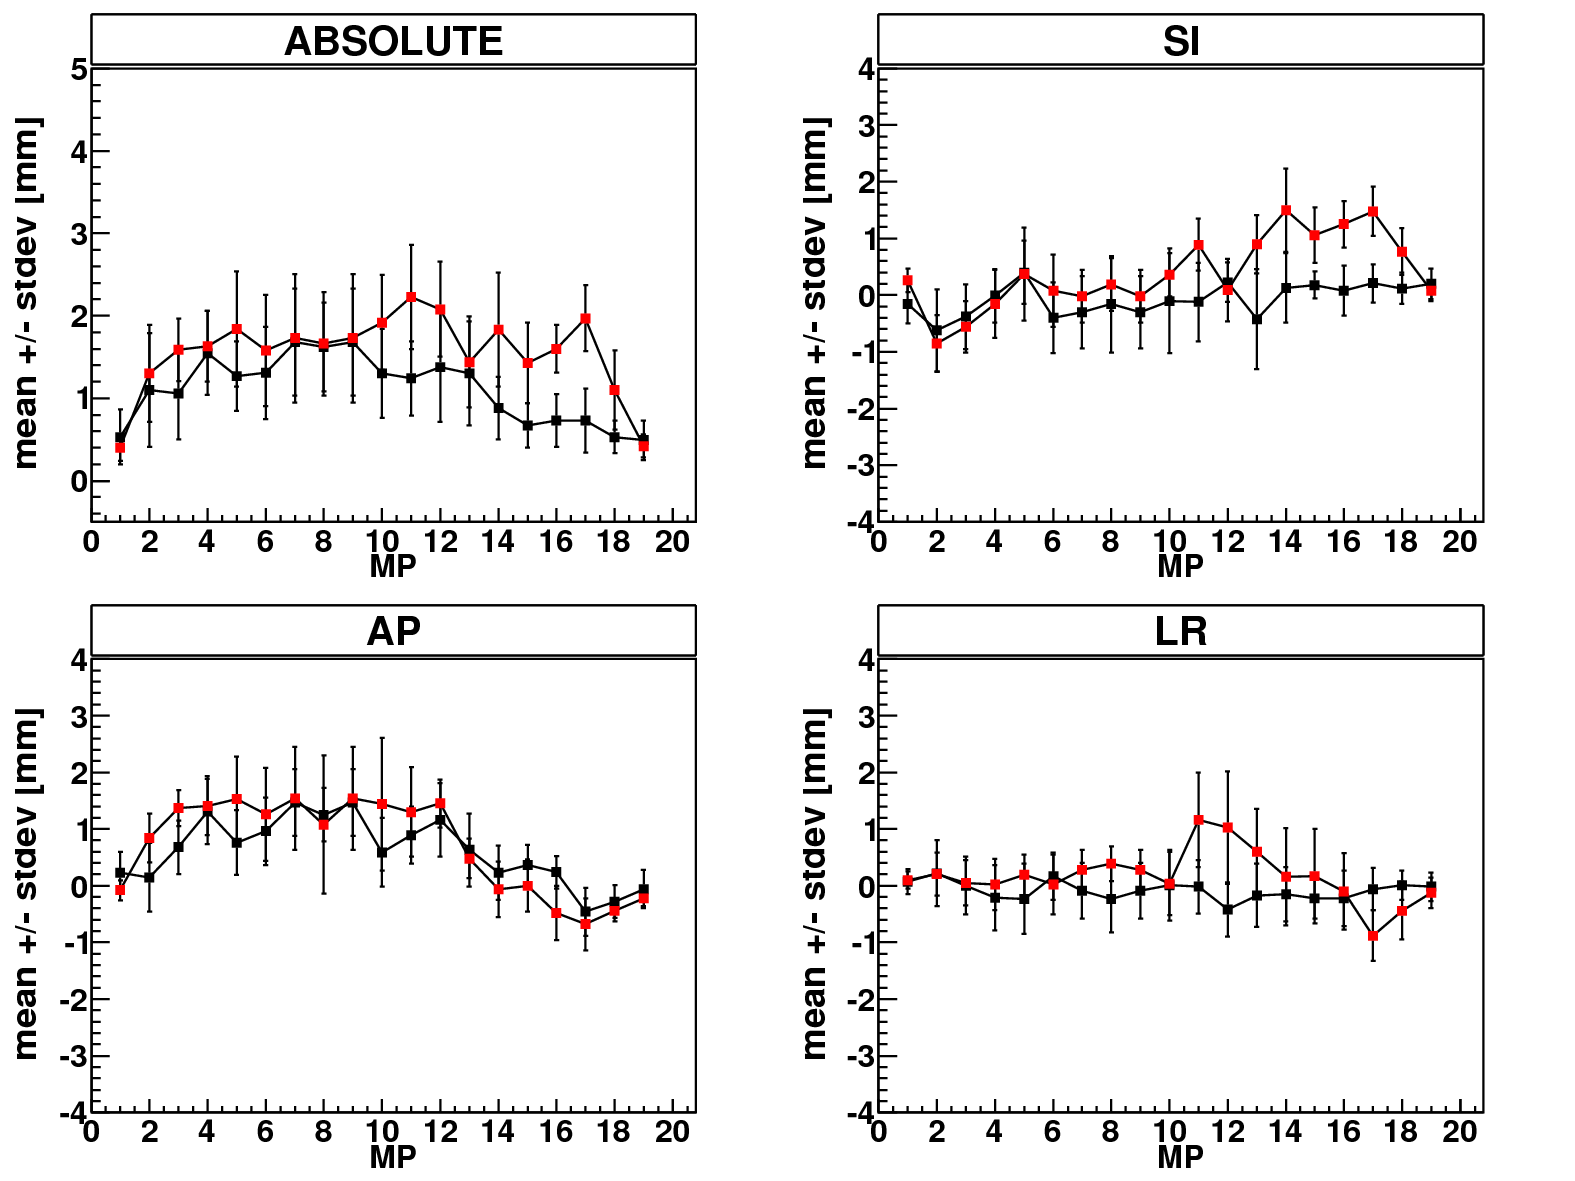
\includegraphics[scale=0.22]{./teile/results_porcine/Mayo_CTI_HB_NATIV_VS_CONTRAST.png}
\caption{CTI: mean motion amplitude and standard deviation in each motion phase (MP) of the heartbeat relative to the reference phase. 
Comparison between native CT data (black) and contrast CT (red) for Pig 3.}
\label{motion_hb_cti_contrast_native}
\end{center}
\end{figure}

\newpage

% \vspace*{-0.5cm}

\begin{figure}[H]
\begin{center}
 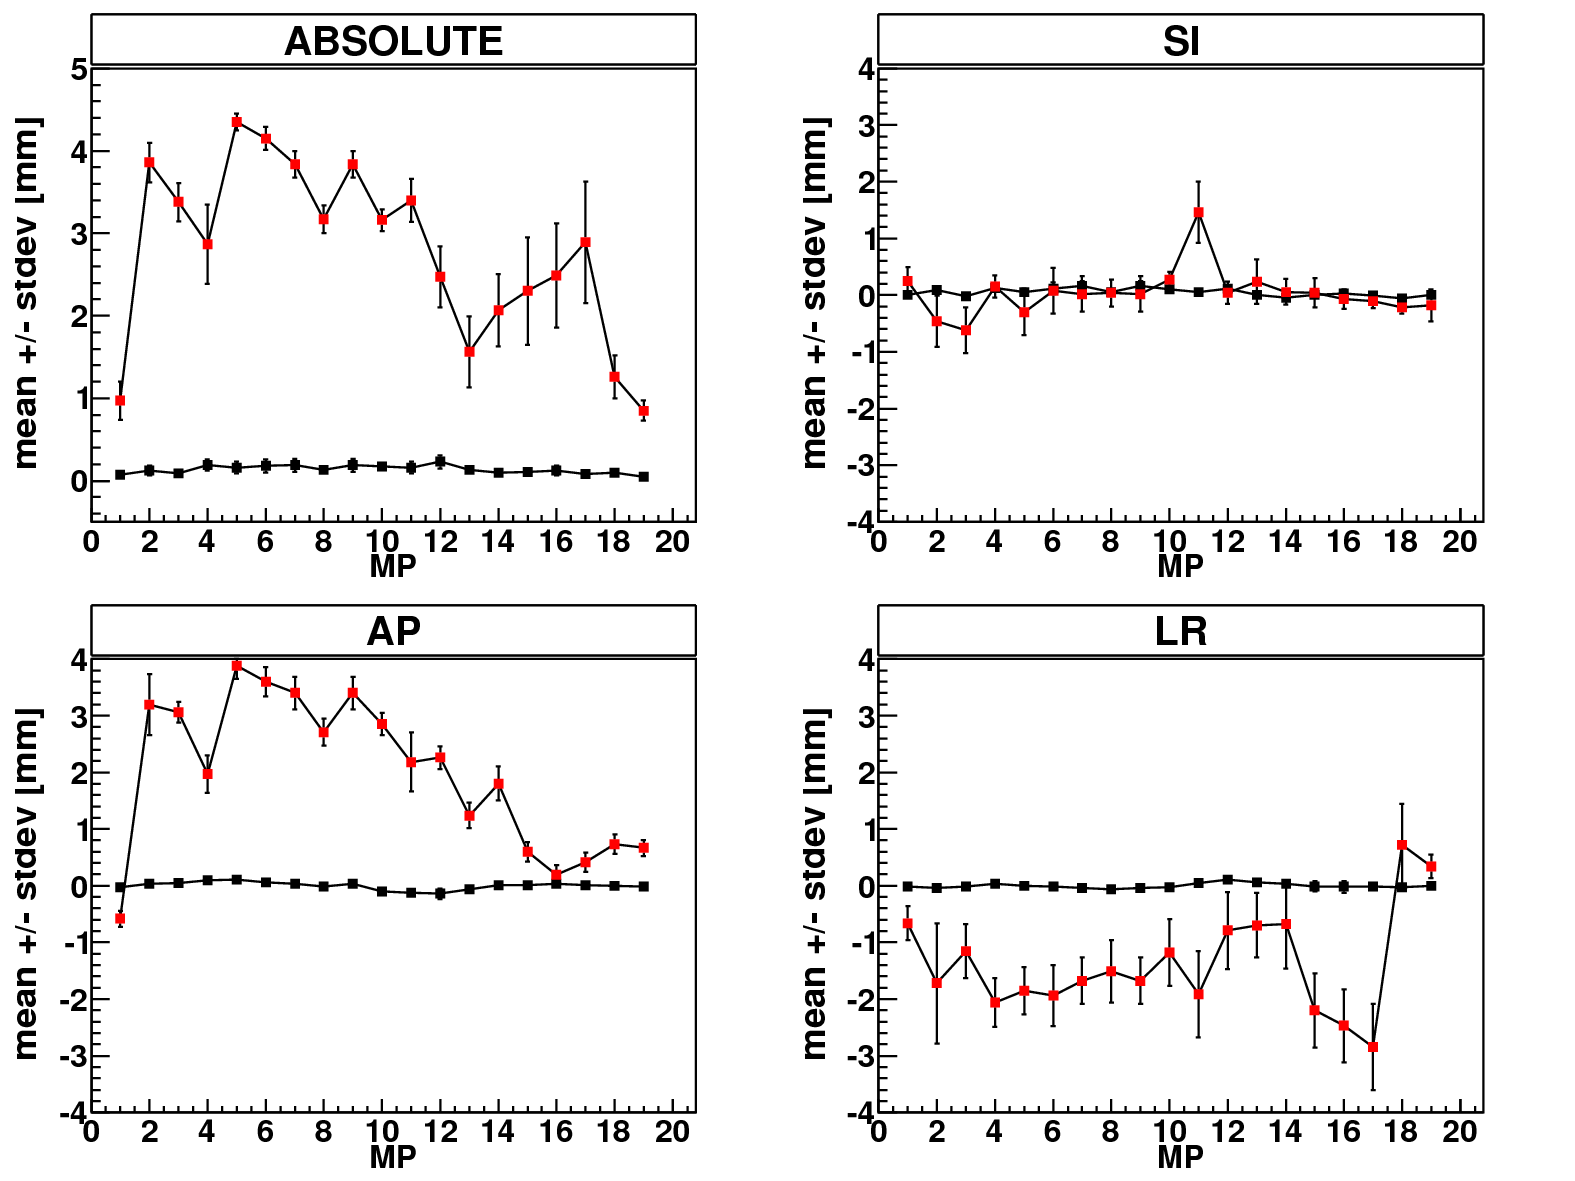
\includegraphics[scale=0.22]{./teile/results_porcine/Mayo_AV_HB_NATIV_VS_CONTRAST.png}
\caption{AV: mean motion amplitude and standard deviation in each motion phase (MP) of the heartbeat relative to the reference phase. 
Comparison between native CT data (black) and contrast CT (red) for Pig 3.}
\label{motion_hb_av_contrast_native}
\end{center}
\end{figure}


% \newpage


\subsubsection*{Motion of cardiac target volumes due to heartbeat}
\label{Sec:Motion_pigs}

% \vspace*{-0.4cm}

The mean and standard deviation over all target volume voxels of the contrast enhanced CTs are plotted for each motion phase and for all pigs 
and motion directions in figure \ref{fig:motion_hb_all_pv} to \ref{fig:motion_hb_all_av}. The numerical values can be found 
in appendix \ref{app:pigs:mmt}. It can be seen that the displacement within the cardiac target volume varies dependent on the studied pig and 
are hence dependent on the underlying anatomy. Furthermore the highest absolute displacement can be observed in different pigs, depending on 
the studied target volume. While the PVs move the most in pig 1 with a displacement of up to 5mm, pig 2 has the 
largest motion both in CTI and AV node (more than 6mm in both structures, respectively) (see also table \ref{tab:maxabsmotion_allpigs}). 
In this table it can be seen that the maximal absolute displacement varies depending on the studied volume. The  
CTI moves with a bigger amplitude than the other two target volumes in three of the four studied pigs (difference found in pig 3). 
The smallest displacement is found in the PVs, again in three of the four studied data sets (again the difference is found in pig 3). 
This can be interpreted in connection to the placement of the target volumes within the heart. While the PVs are found in the upper part of the 
atria, the CTI is located in the lower part of the atria and hence the influence of the ventricular motion should be bigger. The AV node is in between 
the atria and ventricles and was found to have an intermediate absolute displacement in most cases (exception in pig 3).
Independent of the studied target volume the largest contribution to the absolute displacement is found in AP direction for all pigs 
(see table \ref{tab:motion_allpigs}). This can also be seen in the mean displacements over all pigs. 
For the PVs the mean amplitude in SI direction is (0.3 $\pm$ 0.8)mm, (1.5 $\pm$ 1.1)mm in AP direction and (-0.5 $\pm$ 1.0)mm in LR 
direction. In case of the CTI the mean amplitude in SI is (0.8 $\pm$ 0.7)mm, (1.8 $\pm$ 0.7)mm in AP and (0.5 $\pm$ 0.9)mm in LR. For 
the AV node it is (0.7 $\pm$ 0.3)mm in SI, (2.4 $\pm$ 0.4)mm in AP and (-0.7  $\pm$ 0.5)mm in LR. On average, the absolute amplitude 
over all motion phases and pigs is found to (2.3 $\pm$ 0.8)mm for the PVs, (2.8 $\pm$ 0.7)mm for CTI and (3.0 $\pm$ 0.4)mm for the AV node.\newline
\newline
It can be seen in table \ref{tab:maxabsmotion_allpigs} that no motion phase can be directly connected to the maximal absolute 
displacement of the target volumes. As stated in \ref{human:motionheart} the maximal displacement of the atria should thus be observed in 
motion phase eighteen, while the maximal amplitude of the ventricle should be observed in motion phase three. 
While this pattern is not directly connected to the motion of the cardiac volumes it can nevertheless be seen that for all pigs the 
displacement in the biggest motion direction (AP) results in a shallower motion in between MP 6 and 13 compared to the other MPs. 
For the PVs the motion in pig 1 (pig with the largest motion in this target volume) has a range of less than 0.5mm in the interval between MP 
6 and 13, while the motion ranges more than 3mm in the other MPs (see appendix \ref{app:pigs:motion}). The same can be observed in case of the 
CTI, where pig 2 has a less shallow motion range of about 2mm within MP 6 and 13, but nevertheless a larger motion range of up to 4mm in the 
other MPs. Also for the AV node the motion within the MP interval (6-13) is lower (up to 2mm) compared to the the other MPs (range of about 
4.5mm) in pig 2. 

\vspace*{0.8cm}

\begin{table}[H]
  \centering
  \caption{Biggest absolute displacement of target volumes for all pigs with corresponding motion phase.}
  \begin{tabular}{|c|c|c|c|c|}
    \hline\hline
    Target & Pig 1 [mm] (MP) & Pig 2 [mm] (MP) & Pig 3 [mm] (MP) & Pig 4 [mm] (MP) \\
    \hline
    PVs & 4.2 $\pm$ 1.1 (13) & 3.7 $\pm$ 1.6 (12) & 2.4 $\pm$ 0.9 (06) & 3.1 $\pm$ 1.0 (11) \\
    CTI & 5.8 $\pm$ 1.0 (07) & 6.3 $\pm$ 0.5 (08) & 2.2 $\pm$ 0.6 (11) & 4.0 $\pm$ 0.8 (13) \\
    AV & 4.9 $\pm$ 0.3 (13) & 6.0 $\pm$ 0.2 (11) & 4.4 $\pm$ 0.1 (05)  & 3.6 $\pm$ 0.7 (10) \\
    \hline\hline
  \end{tabular}
  \label{tab:maxabsmotion_allpigs}
\end{table}


\newpage

\begin{table}[H]
  \centering
  \small
  \caption{Mean displacement of target volumes over all motion phases for all pigs and motion directions.}
  \begin{tabular}{|c|c|c|c|c|c|}
    \hline\hline
    Target & Pig & ABS [mm] & SI [mm] & AP [mm] & LR [mm] \\
    \hline
    PVs & 1 & 2.9 $\pm$ 0.7 & 0.2 $\pm$ 1.0 & 2.0 $\pm$ 1.3 & -1.1 $\pm$ 1.1 \\
    & 2 & 2.3 $\pm$ 0.9 & 0.9 $\pm$ 0.9 & 1.4 $\pm$ 1.7 & -0.6 $\pm$ 1.0 \\
    & 3 & 1.7 $\pm$ 0.8 & -0.2 $\pm$ 0.6 & 0.7 $\pm$ 0.9 & 0.1 $\pm$ 0.8 \\
    & 4 & 2.1 $\pm$ 0.6 & 0.3 $\pm$ 0.4 & 1.8 $\pm$ 0.7 & -0.2 $\pm$ 0.7 \\
    \hline\hline
    & Pig & ABS [mm] & SI [mm] & AP [mm] & LR [mm] \\
   \hline
    CTI & 1 & 3.5 $\pm$ 0.8 & 0.7 $\pm$ 0.8 & 2.3 $\pm$ 0.8 & 1.5 $\pm$ 0.9 \\
    & 2 & 3.5 $\pm$ 0.8 & 1.0 $\pm$ 1.0 & 2.4 $\pm$ 0.5 & 0.3 $\pm$ 1.2 \\
    & 3 & 1.6 $\pm$ 0.6 & 0.4 $\pm$ 0.5 & 0.7 $\pm$ 0.7 & 0.2 $\pm$ 0.6 \\
    & 4 & 2.1 $\pm$ 0.5 & 0.8 $\pm$ 0.4 & 1.7 $\pm$ 0.5 & 0.0 $\pm$ 0.5 \\
    \hline\hline
   & Pig & ABS [mm] & SI [mm] & AP [mm] & LR [mm] \\
   \hline
    AV & 1 & 3.0 $\pm$ 0.4 & 0.4 $\pm$ 0.4 & 2.5 $\pm$ 0.5 & -0.7 $\pm$ 0.4 \\
    & 2 & 3.7 $\pm$ 0.4 & 1.9 $\pm$ 0.3 & 3.0 $\pm$ 0.3 & 0.1 $\pm$ 0.4 \\
    & 3 & 2.8 $\pm$ 0.4 & 0.0 $\pm$ 0.3 & 2.0 $\pm$ 0.3 & -1.4 $\pm$ 0.6 \\
    & 4 & 2.1 $\pm$ 0.4 & 0.5 $\pm$ 0.2 & 1.7 $\pm$ 0.3 & -0.7 $\pm$ 0.4 \\
    \hline\hline
  \end{tabular}
  \label{tab:motion_allpigs}
\end{table}

\vspace*{0.4cm}

\begin{figure}[H]
\begin{center}
 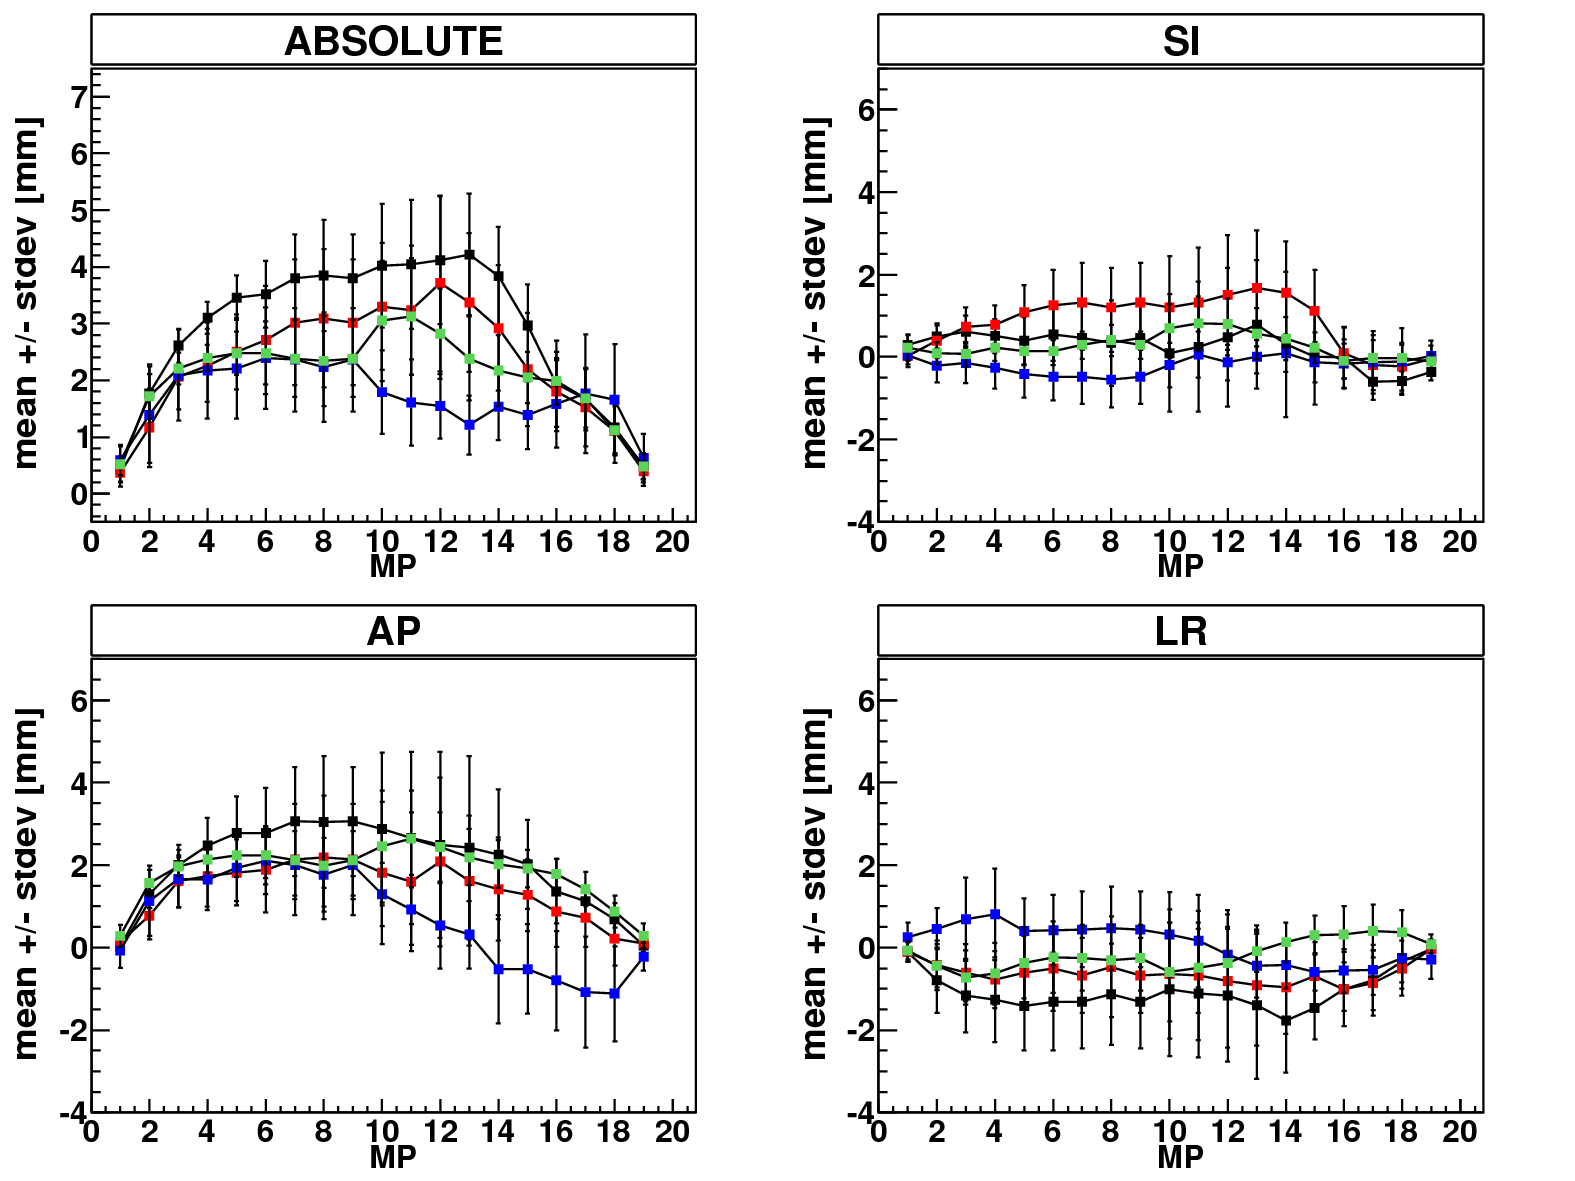
\includegraphics[scale=0.22]{./teile/results_porcine/Mayo_PV_HB.png}
\caption{PVs: Mean motion amplitude and standard deviation in each motion phase (MP) under influence of heartbeat for all porcine, obtained 
from contrast enhanced CT scans. (pig 1: black, pig 2: red, pig 3: blue, pig 4: green) }
\label{fig:motion_hb_all_pv}
\end{center}
\end{figure}

\newpage

\begin{figure}[H]
\begin{center}
 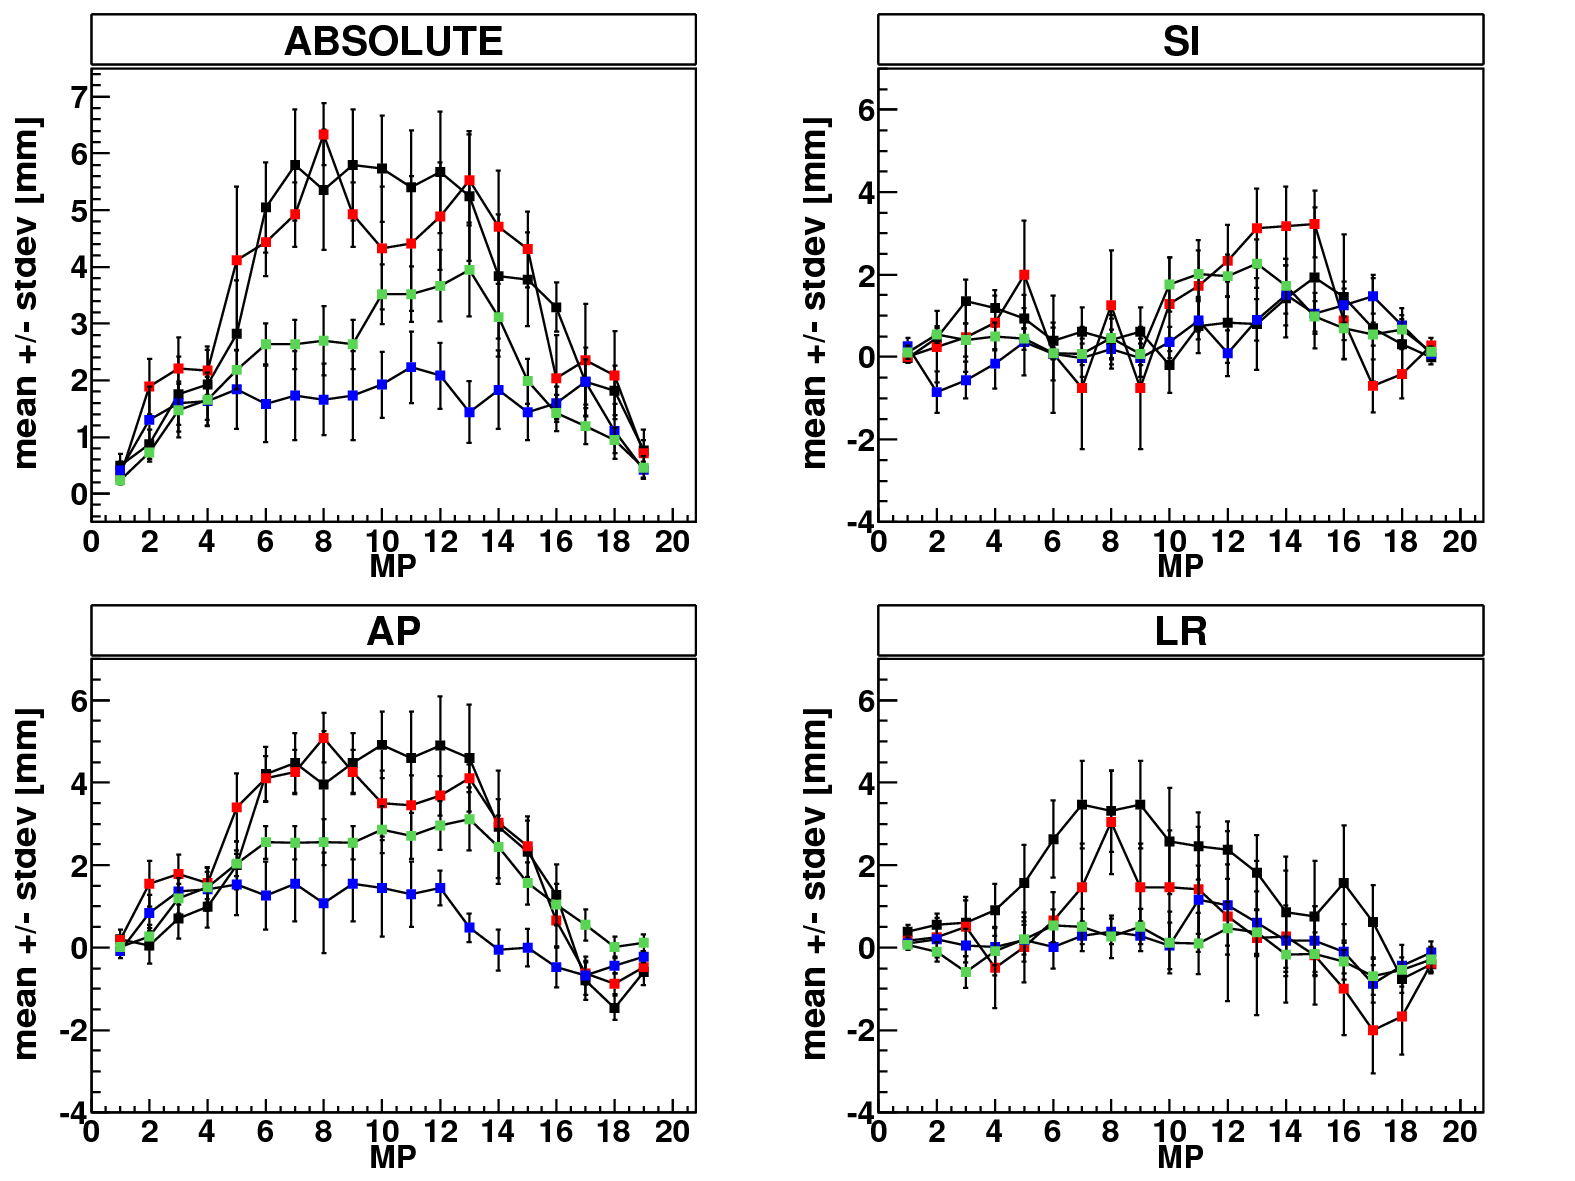
\includegraphics[scale=0.22]{./teile/results_porcine/Mayo_CTI_HB.png}
\caption{CTI: Mean motion amplitude and standard deviation in each motion phase (MP) under influence of heartbeat for all porcine, obtained 
from contrast enhanced CT scans. (pig 1: black, pig 2: red, pig 3: blue, pig 4: green) }
\label{fig:motion_hb_all_cti}
\end{center}
\end{figure}

% \newpage
\vspace*{-0.4cm}

\begin{figure}[H]
\begin{center}
 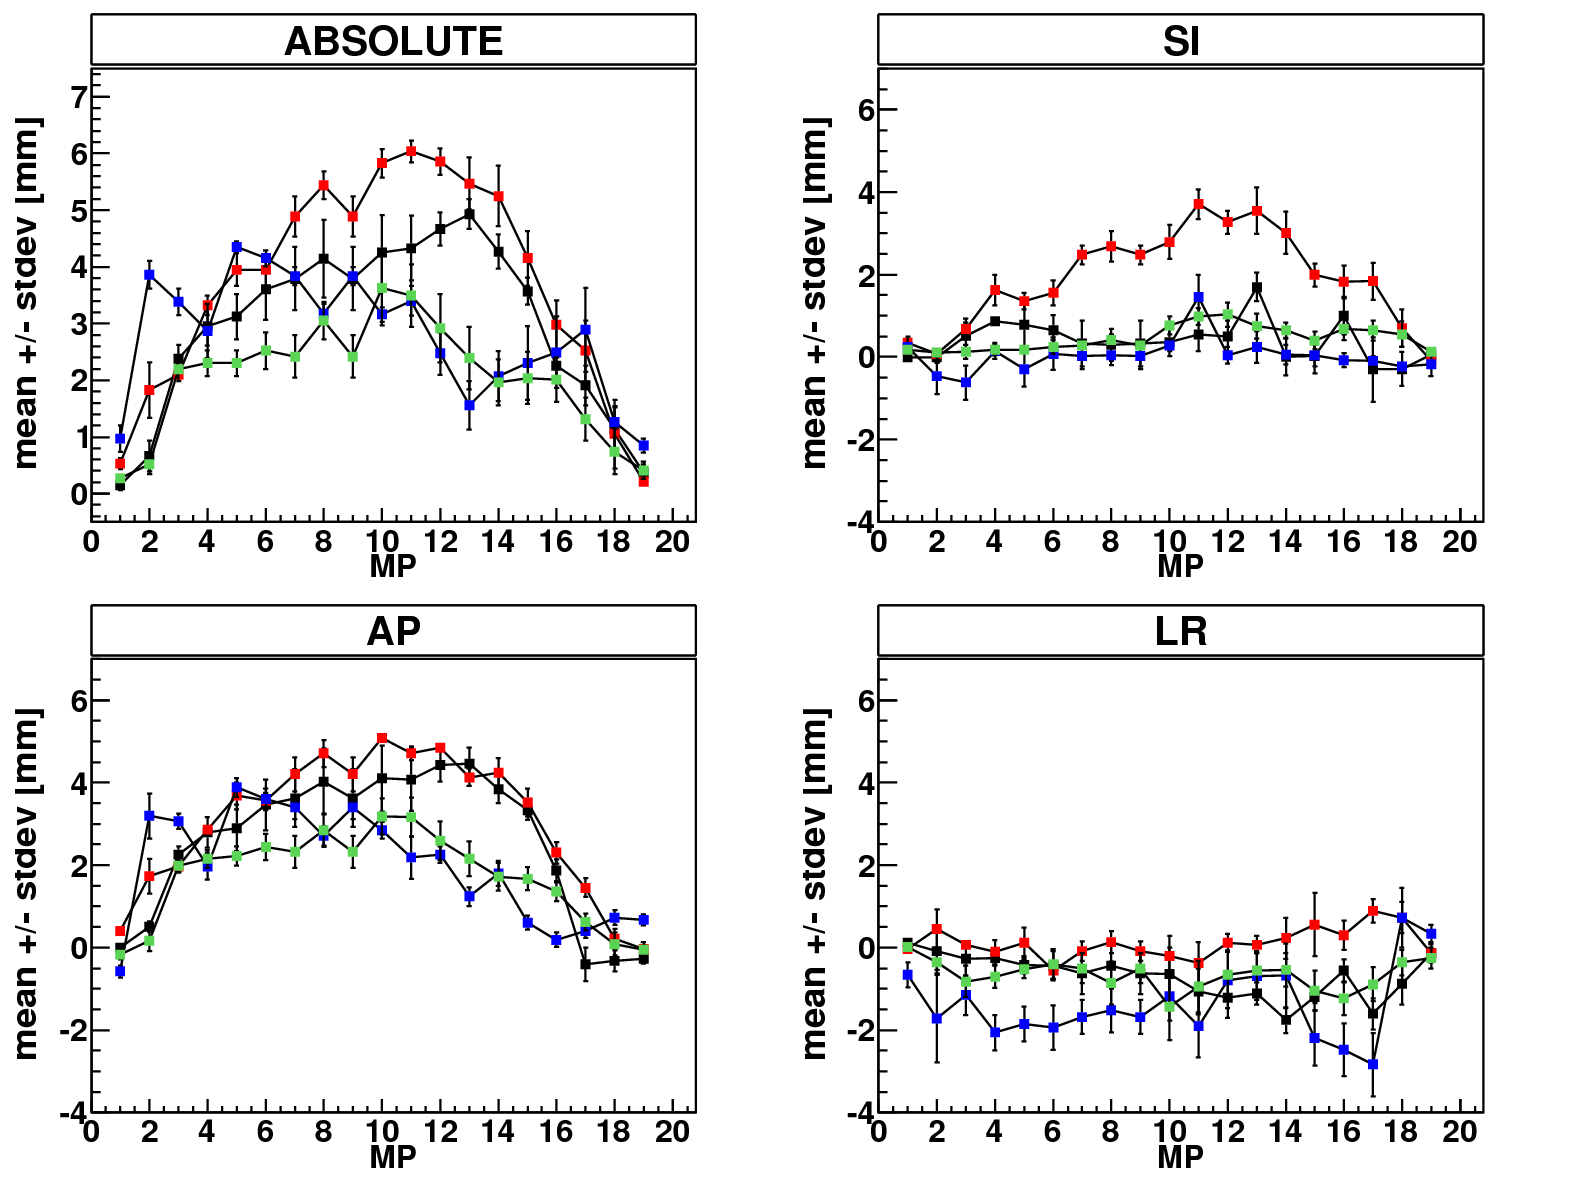
\includegraphics[scale=0.22]{./teile/results_porcine/Mayo_AV_HB.png}
\caption{AV node: Mean motion amplitude and standard deviation in each motion phase (MP) under influence of heartbeat for all porcine, 
obtained from contrast enhanced CT scans. (pig 1: black, pig 2: red, pig 3: blue, pig 4: green) }
\label{fig:motion_hb_all_av}
\end{center}
\end{figure}

\newpage

The overall displacement field for two exemplary pigs with a small motion amplitude (pig 4) and a large motion amplitude (pig 2) of the 
AV node are shown in figure \ref{contour_plot_hb_pigs}. The field is shown for the maximal displacement motion phase of the respective pigs 
(motion phase 11 for pig 2 and motion phase 10 for pig 4, see table \ref{tab:maxabsmotion_allpigs}). 
In order to visualize the location of the displacement, an axial cut of the reference state CT is 
underlayed. The absolute values of the displacement vectors are shown as contour plots. 


\begin{figure}[H]
\centering
\subfigure[Pig 2: max. abs. motion (MP 11)]{
 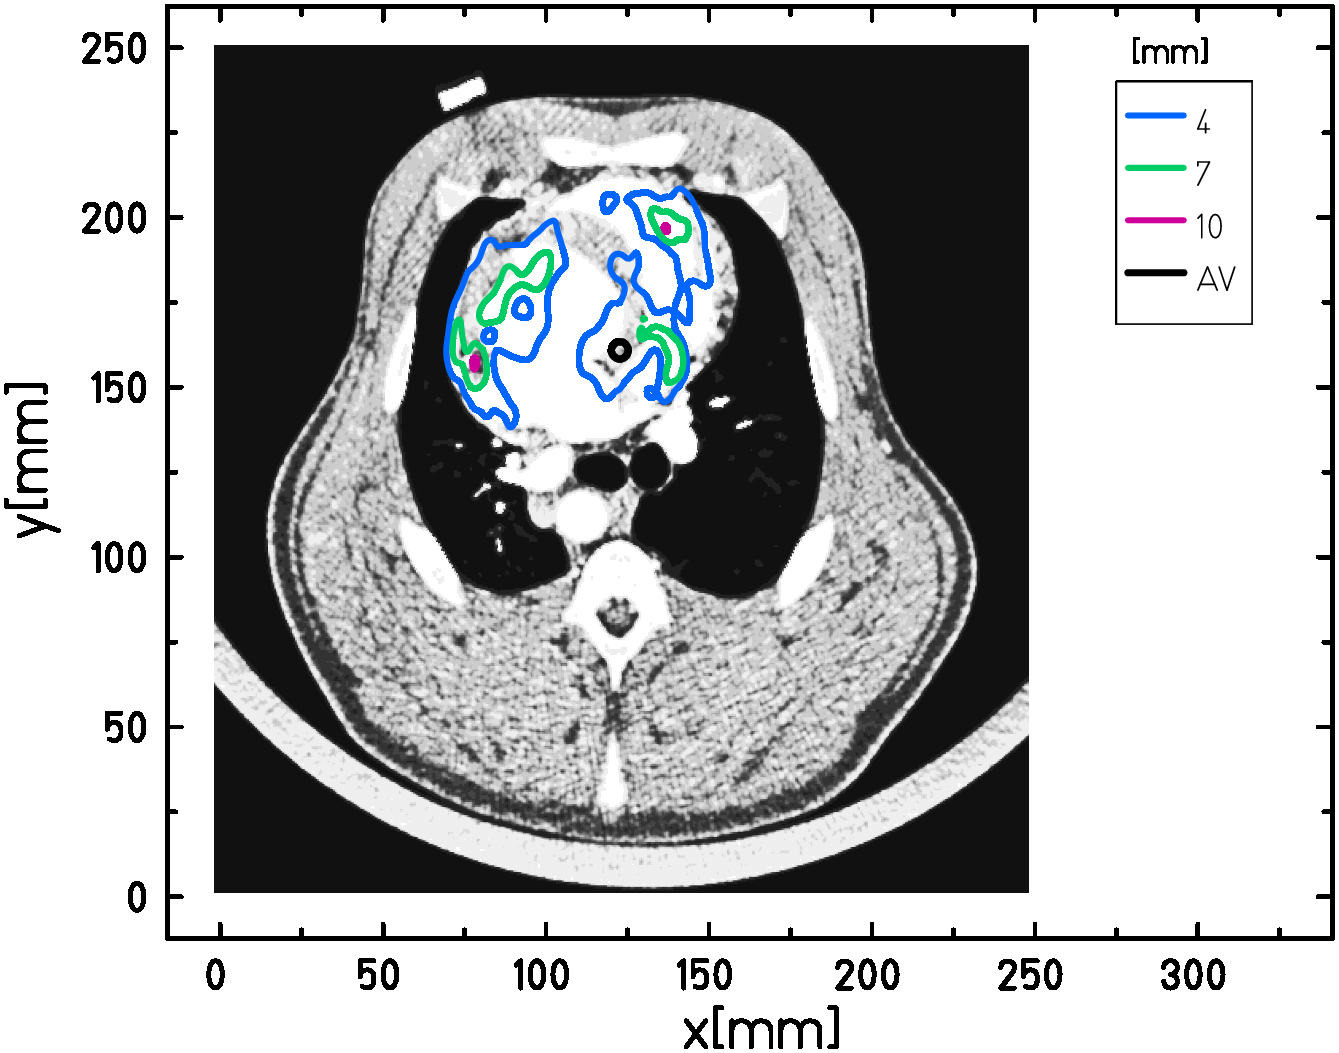
\includegraphics[scale=0.2]{./teile/results_porcine/Contour_z_abs_HB_L833_11_HUskala_gedreht.png}
}
\subfigure[Pig 4: max. abs. motion (MP 10)]{
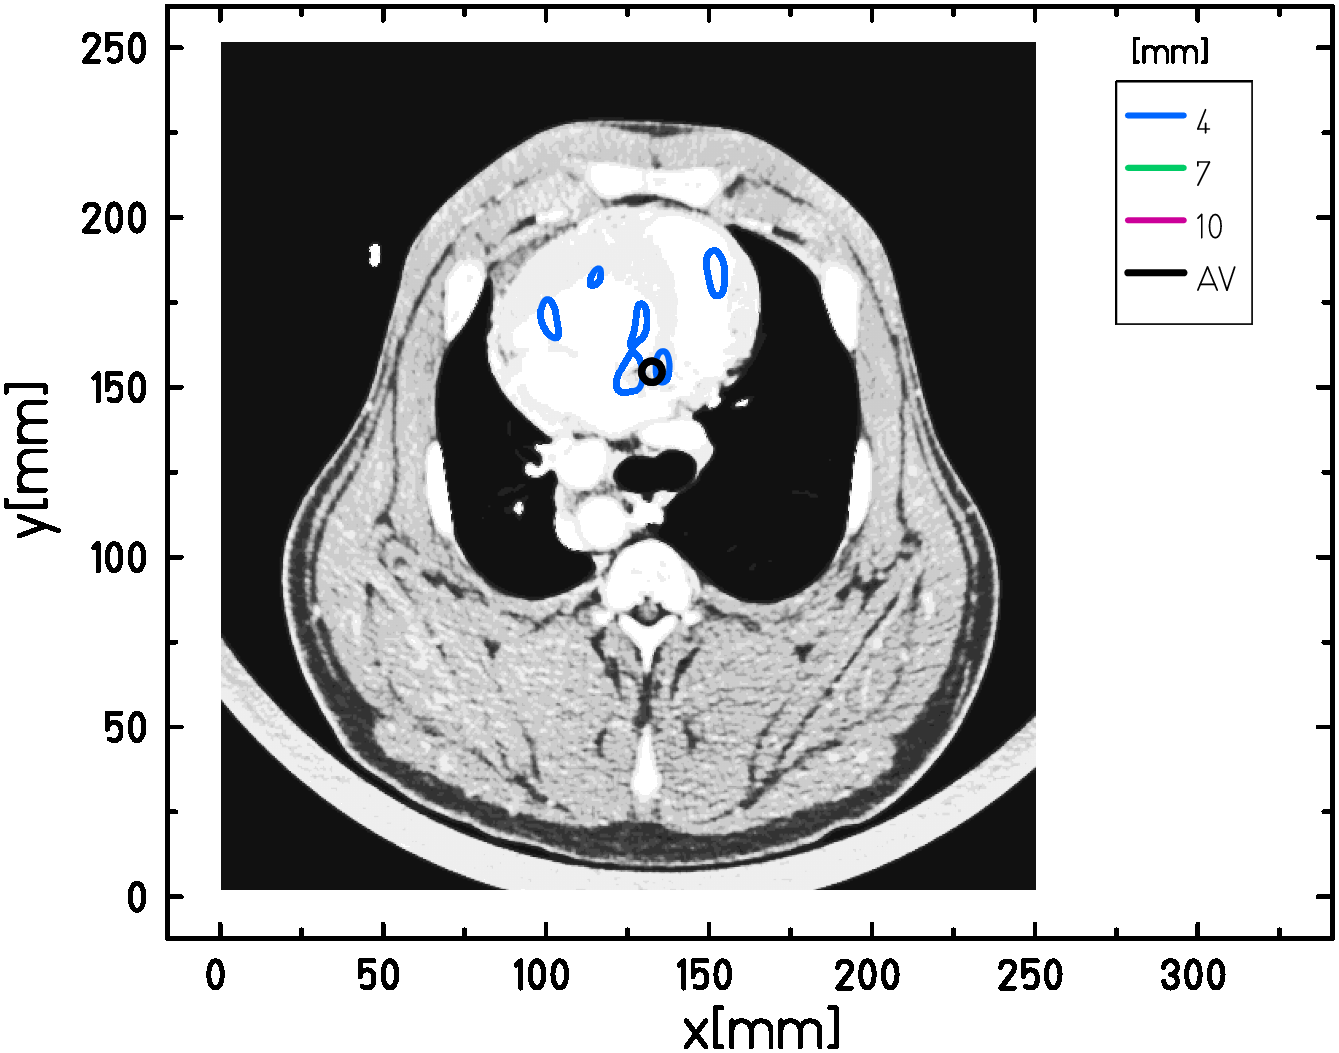
\includegraphics[scale=0.2]{./teile/results_porcine/Contour_z_abs_HB_L979_10_HUskala_gedreht.png}
}
\caption{Axial slices of the reference state of the CT overlayed with the absolute values of the displacement field (obtained from 
deformable image registration) in the corresponding slice for heartbeat motion. Above: the resulting displacement of pig 2 is shown 
in MP 11. Below: the results for pig 4 in MP 10.}
\label{contour_plot_hb_pigs}
\end{figure}
 
\newpage


\subsection{Dose to organs at risk when irradiating the AV node}

Due to the fact that the AV node is located in a large distance to the OARs (see figure \ref{pig1_targets}), the dose deposition in the 
studied structures is not critical. Esophagus, trachea as well as the aorta are receiving no dose in all studied cases. 
Only the heart is receiving up to 7Gy for the studied volume of 15cm$^{3}$. The respective dose-volume limit of 16Gy to 15cm$^{3}$ is hence 
not exceeded.  The dose deposited in the stated heart volume ranges from 4.8Gy (pig 3) to 7.3Gy (pig 4), which corresponds to 19\% and 29\% of 
the physical dose. Hence even higher doses of up to 40Gy would not exceed the dose volume limit. 
The results of a more detailed analysis of the affected cardiac substructures can be seen in table \ref{DV_OAR:pig}. Here the mean dose to the 
whole structure is stated next to the maximal point dose for all pigs and studied structures. Furthermore the maximal irradiated volume 
is shown. 


\begin{table}[htbp]
\footnotesize
\centering
\caption{Mean as well as maximum point dose to the whole heart and different cardiac substructures as well as maximal irradiated 
volume of the structures for all pigs.}
  \begin{tabular}{ |c||c||c|c|c|}
    \hline
    OAR & Pig & Mean dose [Gy] & Max dose [Gy] & Max volume [\%] \\ \hline \hline
Heart & 1 & 0.6 & 25.8 & 14.0 \\ 
 & 2 & 0.5 & 25.4 & 12.7 \\ 
 & 3 & 0.8 & 25.3 & 17.4 \\ 
 & 4 & 0.8 & 25.7 & 16.6 \\ 
\hline
LV & 1 & 0.5 & 26.3 & 6.7 \\ 
 & 2 & 0.5 & 26.3 & 6.1 \\ 
 & 3 & 0.3 & 26.1 & 5.1 \\ 
 & 4 & 0.4 & 26.0 & 4.5 \\ 
\hline
RV & 1 & 0.3 & 25.2 & 9.1 \\ 
 & 2 & 0.2 & 25.2 & 8.0 \\ 
 & 3 & 0.4 & 25.3 & 9.6 \\ 
 & 4 & 0.5 & 25.8 & 14.3 \\ 
\hline
LCA & 1 & 0.8 & 7.4 & 19.9 \\ 
 & 2 & 0.6 & 7.2 & 13.5 \\ 
 & 3 & 0.2 & 6.4 & 8.9 \\ 
 & 4 & 0.7 & 7.4 & 14.6 \\ 
\hline
RCA & 1 & 1.5 & 9.2 & 37.6 \\ 
 & 2 & 1.1 & 8.4 & 24.0 \\ 
 & 3 & 1.4 & 9.8 & 37.3 \\ 
 & 4 & 1.4 & 9.6 & 34.1 \\ 
\hline
  \end{tabular}
  \label{DV_OAR:pig}
\end{table}

Due to the physical dose deposition of 25Gy in the AV node the heart is receiving a relatively high maximum point dose with a median of 
25.6Gy (75th percentile: 25.8Gy) over all pigs. The mean heart dose is found to have a median of 0.7Gy (0.8Gy) and the median of the 
maximal irradiated volume over all porcine data sets is 15.3\% (17.7\%). Comparing the dose deposition in the left and right ventricles 
it can be seen that the maximum point dose is higher in the LV than in the RV, with a median of 26.2Gy (26.3Gy) compared to 25.2Gy (25.5Gy). 
Nevertheless the mean dose is comparable with a median of 0.5Gy (0.5Gy) for the LV and 0.4Gy (0.5Gy) for the RV and the maximal irradiated 
volume is smaller for the LV compared to the RV with a median of 5.6\% (6.4\%) compared to 9.3\% (11.9 \%). It should be noted that the total 
volume of the LV is much larger than the RV (e.g. about three times larger in pig 1), so that the absolute maximal irradiated volume 
results to be larger in case of the LV. Concerning the coronary arteries, 
it can be seen that the mean and maximal point dose to the LCA is smaller than to the RCA, resulting in a median mean dose of 0.6Gy (0.7Gy) 
in LCA compared to 1.4Gy (1.4Gy) in RCA and a median maximum point dose of 7.3Gy (7.4Gy) in LCA compared to 9.4Gy (9.7Gy) in LCA. 
Also the maximal irradiated volume is much smaller in the LCA compared to the RCA, resulting in a median maximum volume of 14.1\% (17.2\%) 
versus 35.7\% (37.5\%). 

\subsection{Motion mitigation techniques for AV node irradition}

The resulting interplay effect, caused by the displacement of the AV node of up to 6mm, and dose deposition were studied for every porcine 
data set for different motion patterns and 5mm margin to the target volume. The dose analysis values V95, V107 and D5-D95 were assessed and 
plotted. For comparison, also the corresponding values for the 3D case (static) are shown. Rescanning was studied as motion mitigation 
technique. The results of the stated dose values in case of rescanning with rescan numbers of five, ten and fifteen will be presented. 


\subsubsection{Dose deposition}
Different motion pattern DVHs of fifteen rescans compared to the interplay results as well as a static irradiation are displayed for pig 2 
(as this is the pig with the largest motion amplitude in the AV node) in figure \ref{dvhs_pig2_pig4} for 5mm safety margin. 
A representative dose deposition for all studied techniques (static, interplay and rescanning with fifteen rescans) is shown exemplary in 
figure \ref{dose_pig2}. Rescanning and interplay are shown for a motion with a period of 0.5s and a starting phase of 90$^{\circ}$. The target 
volume was irradiated with an added margin of 5mm. It can already be seen from this dose cut figures that rescanning with fifteen rescans 
improves the outcome compared to interplay and yields a result which is comparable to the static case. Due to the mechanism of rescanning, the 
field size is slightly increased compared to the static irradiation.\newline
\newline
In order to assess the dose information of all pigs, the DVHs were analyzed and compared for dose steepness, dose coverage as well as over 
dosage. The results for all porcine data sets are shown in figure \ref{static_interplay_rescanning_ALLpigs}. The corresponding numerical 
values can be found in appendix \ref{app:pigs} (tables \ref{tab:Pig1_AV} - \ref{tab:Pig4_AV}).\newline
\newpage
The resulting interplay pattern is dependent on the underlying motion period and starting phase. This can also be seen in the mean values and 
standard deviations of the dose analysis parameters over all pigs  for different motion patterns. The dose coverage for example is found to 
have a mean value of V95=(84.3 $\pm$ 17.5)\% for a motion with 0.7s period and a starting phase of 0$^{\circ}$, while it is found to be (91.0 
$\pm$ 10.3)\% for the same period and a starting phase of 90$^{\circ}$. For a period of 0.5s the mean dose coverage over all pigs is found to 
be (84.5 $\pm$ 8.0)\% with a phase of 0$^{\circ}$ and to (86.0 $\pm$ 24.0)\% for a phase of 90$^{\circ}$. The resulting high standard deviation 
shows that the result is also dependent on the studied porcine case.These dependencies are also valid for the other studied dose analysis 
parameters, dose homogeneity and over dosage.\newline
\newline
It can furthermore be seen in figure \ref{static_interplay_rescanning_ALLpigs} (as well as numerical values for all pigs in appendix \ref{app:pigs:motion}) 
that rescanning can improve the results for dose steepness, dose coverage as well as over dosage compared to the interplay case in all studied 
motion cases for three out of four pigs. Only pig 2, which was found to have the largest absolute displacement of the AV node out of the four 
studied porcine data sets, results in some rescanning cases where slightly inferior results compared to interplay are achieved. This is the 
case in dose steepness, where a motion with 0.7s and 90$^{\circ}$ starting phase is D5-D95=8.2\% with five rescans and D5-D95=7.9\% 
with ten rescans compared to D5-D95=6.2\% without any compensation (interplay). For the same motion the dose coverage is found to be V95=43.6\% 
with five rescans compared to V95=99.0\% with interplay. This result can already be improved with ten rescans, where V95 is found to be 98.5\%.  
In over dosage a motion pattern (period of 0.5s and starting phase of 0$^{\circ}$) is found to have inferior results with ten rescans compared 
to interplay (9.3\% versus 0\%). The results for ten rescans could be slightly improved with fifteen rescans, so that, e.g., 
the dose coverage is found to be V95=100\% for the stated motion pattern (0.7s period and 90$^{\circ}$ starting phase) (static: 100\%). 
For pig 4, which has the smallest absolute displacement of the AV node in the studied porcine cohort, all rescanning results yield 
improved results compared to interplay. Moreover it can also be observed here that ten and fifteen rescans result in better dose analysis 
parameters and even tops the static outcome in some cases. E.g. the dose steepness is found to be D5-D95=3.0\% with a motion period of 0.5s 
and starting phase of 0$^{\circ}$ for fifteen rescans and to be 5.1\% with ten rescans, while in the static case it is found to be 5.5\%. 
In this case also five rescans result in an improved dose steepness (D5-D95=4.9\%). 
Regarding the dose coverage, fifteen rescans yield results comparable to the static case (100\%) for all motion patterns, while ten rescans 
yield comparable results (e.g. 97.8\% for motion period of 0.7s and starting phase of 90$^{\circ}$, interplay: 74.3\%). Five rescans 
on the other hand show inferior results with, e.g., D5-D95=86.3\% for a motion period of 0.5s and a starting phase of 0$^{\circ}$.\newline  

\newpage

\vspace*{0.8cm}

 \begin{figure}[H]
 \begin{center}
\subfigure[pig 2]{
 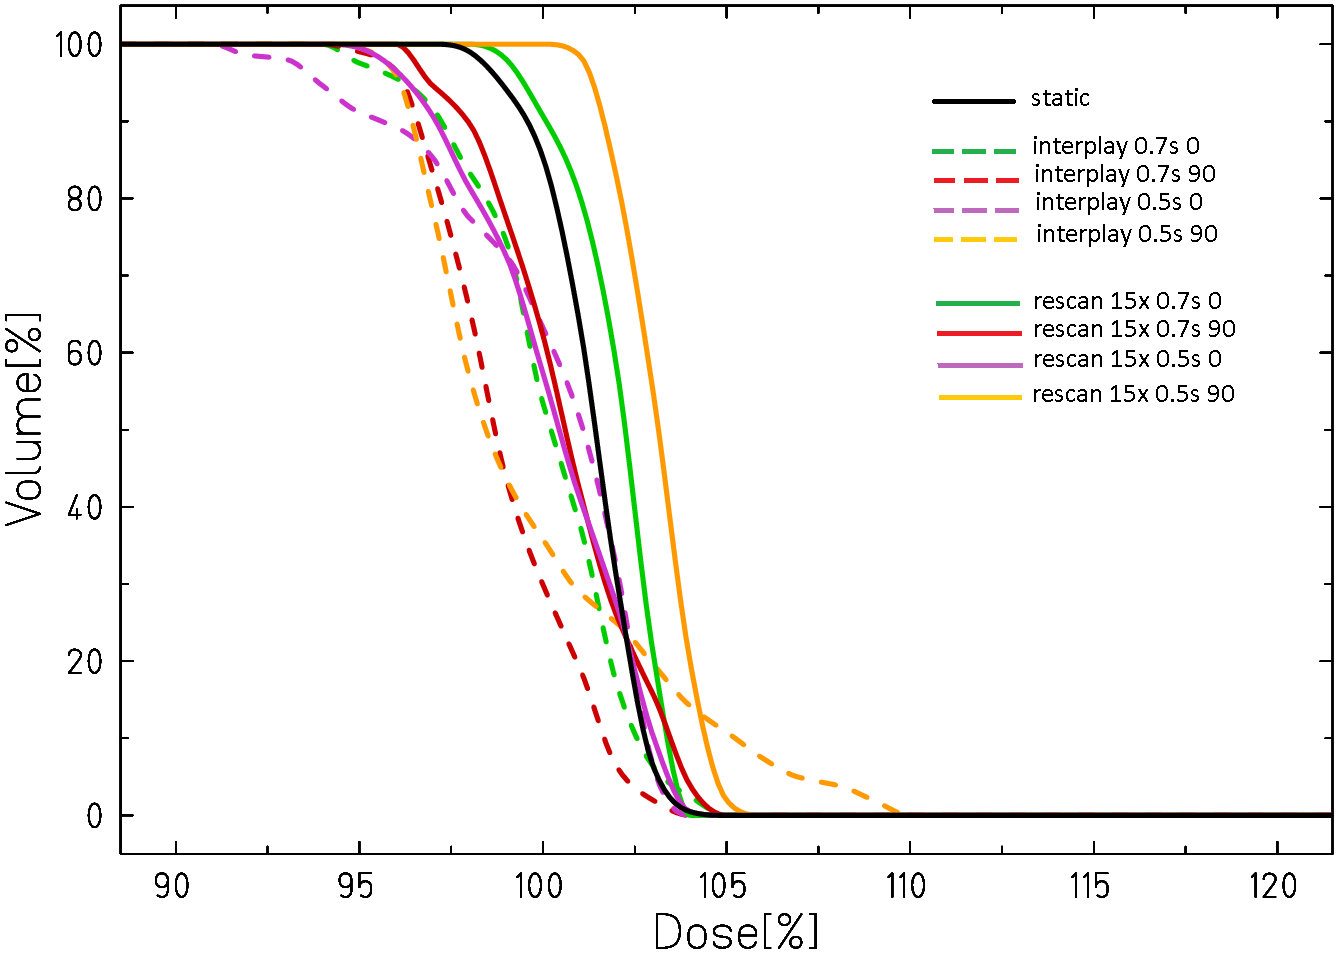
\includegraphics[scale=0.28]{./teile/results_porcine/L833_AV_allDVHs_withLegend.png}
 }
\subfigure[pig 4]{
 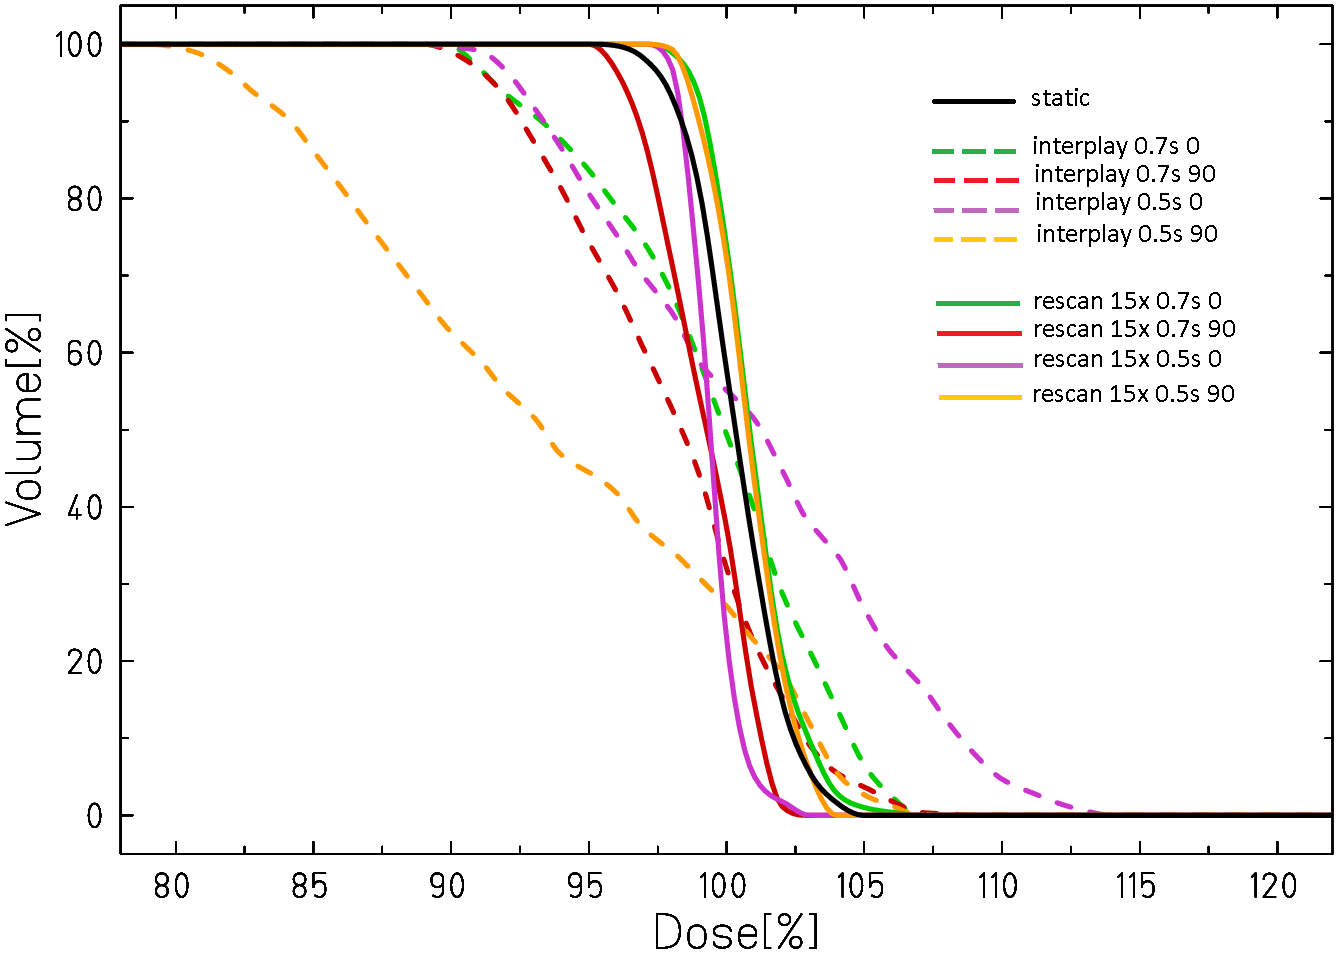
\includegraphics[scale=0.28]{./teile/results_porcine/L979_AV_allDVHs_withLegend.png}
 }
\caption{Dose volume histograms for CTV of pig 2 (largest absolute displacement of AV node) and pig 4 (smallest absolute displacement of AV 
node) for 5mm safety margin irradiation of AV node in case of static irradiation (black), interplay (dashed) and rescanning with fifteen 
rescans (solid). The motion patterns are shown in colors (0.7s 0: motion period of 0.7s and starting phase 0$^{\circ}$, 0.7s 90: motion period 
of 0.7s and starting phase 90$^{\circ}$, 0.5s 0: motion period of 0.5s and starting phase 0$^{\circ}$, 0.5s 90: motion period of 0.5s and 
starting phase 90$^{\circ}$).}
\label{dvhs_pig2_pig4}
 \end{center}
\end{figure}


\newpage

\vspace*{0.4cm}


 \begin{figure}[H]
 \begin{center}
 \centering
\subfigure[static]{
 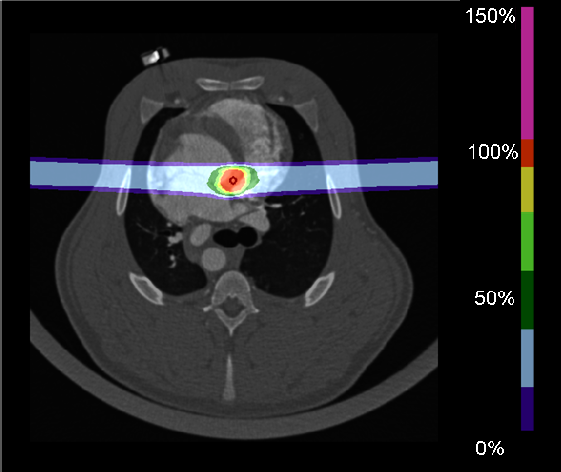
\includegraphics[scale=0.56]{./teile/results_porcine/Mayo_Pig_L833_contrast_STATIC_withLegend.png}
 }
\subfigure[interplay]{
 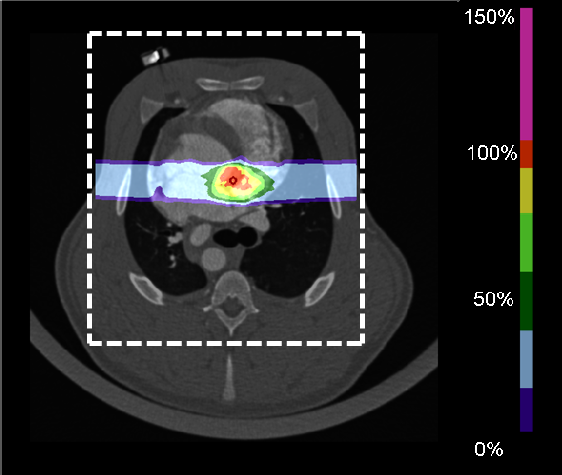
\includegraphics[scale=0.56]{./teile/results_porcine/Mayo_Pig_L833_contrast_INTERPLAY_sin05s90_withLegend.png}
 }
 \subfigure[rescanning (15x)]{
 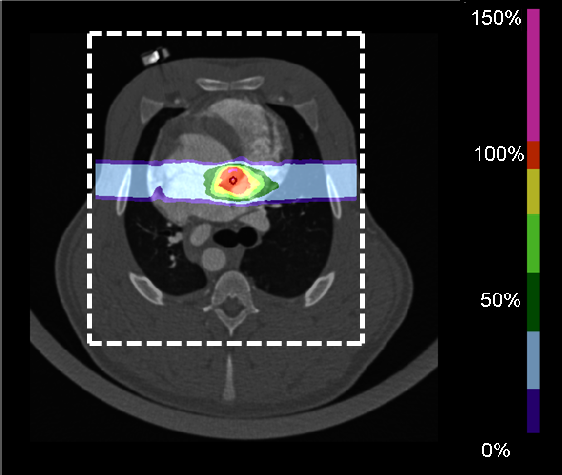
\includegraphics[scale=0.56]{./teile/results_porcine/Mayo_Pig_L833_contrast_RESCANNING_15x_sin05s90_withLegend.png}
 }
\caption{Dose distribution of pig 2 for static (a) as well as interplay (b) and fifteen rescans (c) at motion period of 0.5s and a motion 
starting phase of 90$^{\circ}$. The target volume has an added margin of 5mm. The improved outcome of rescanning compared to interplay 
can already be seen in these dose cuts. For interplay and rescanning the dose was calculated in a reduced volume as indicated by the white 
dashed line.}
\label{dose_pig2}
 \end{center}
\end{figure}

\newpage

\begin{figure}[H]
\centering
\subfigure[D5-D95]{
 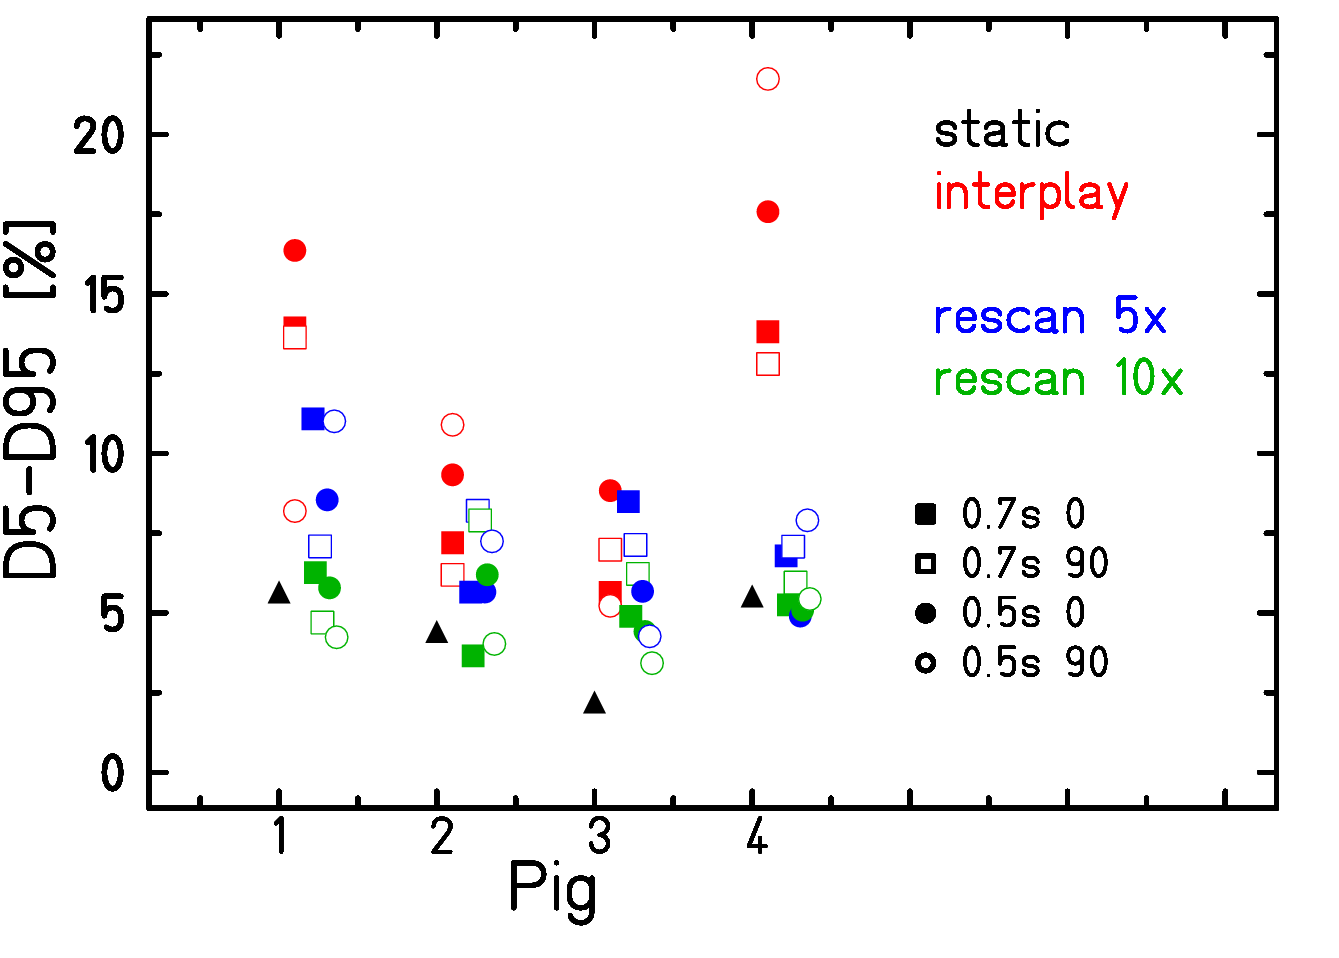
\includegraphics[scale=0.18]{./teile/results_porcine/MAYO_CTV_AV_D5D95.png}
 }
 \subfigure[V95]{
 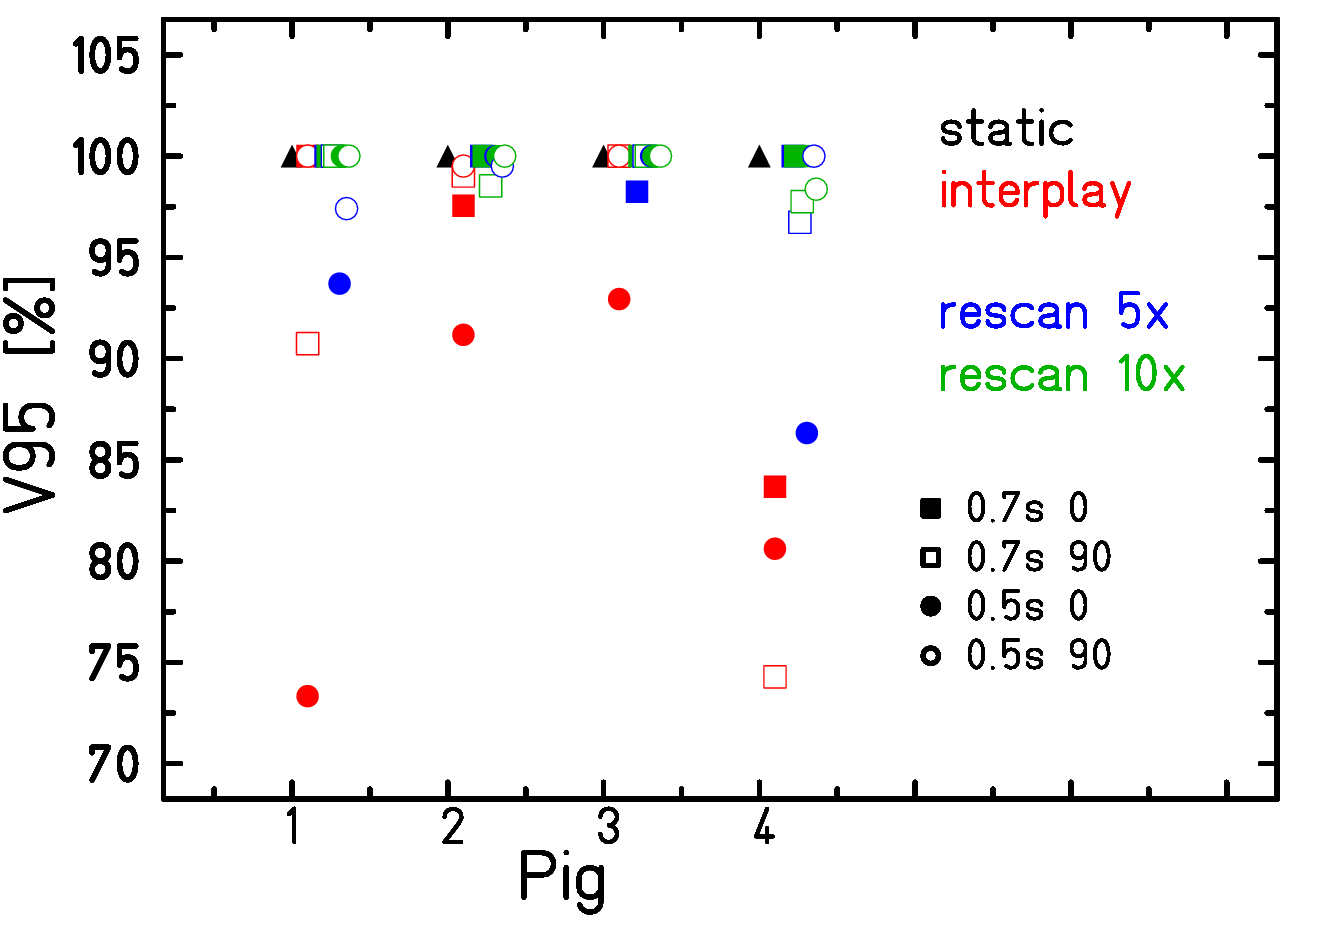
\includegraphics[scale=0.18]{./teile/results_porcine/MAYO_CTV_AV_V95.png}
 }
  \subfigure[V107]{
 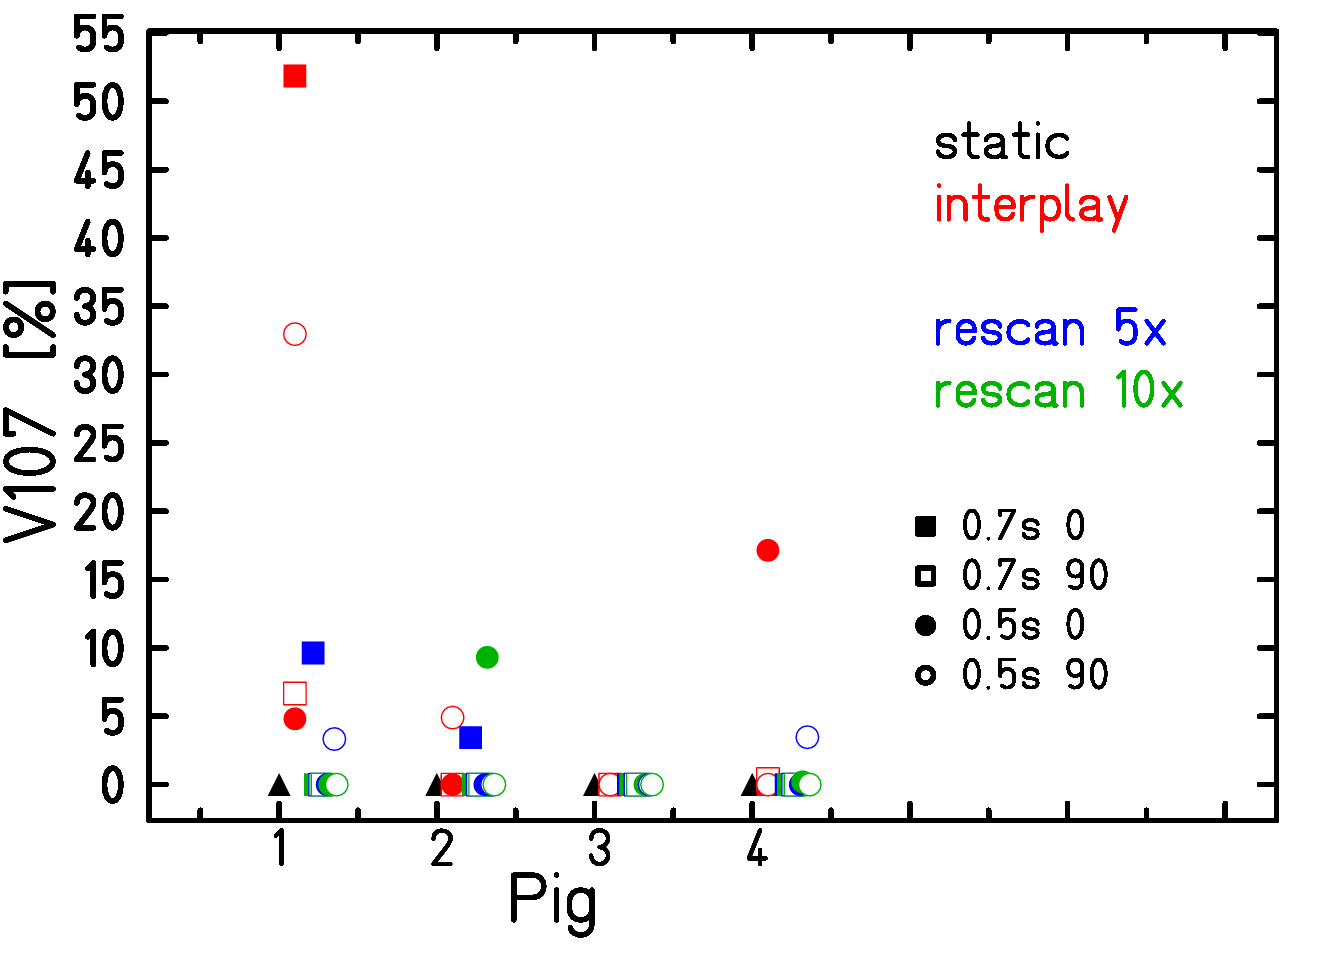
\includegraphics[scale=0.18]{./teile/results_porcine/MAYO_CTV_AV_V107.png}
}
\caption{Dose analysis parameters D5-D95 (first row), V95 (middle row) and V107 (last row) for all porcine data sets when irradiating the AV 
node with 5mm safety margin. Static (black) as well as interplay (red) and different rescanning numbers (5 times: blue, 10 times: green,) were 
compared for different motion patterns and safety margins. For a better visualization the rescanning data points for each motion pattern are 
shifted and the results for fifteen rescans are not displayed.}
\label{static_interplay_rescanning_ALLpigs}
\end{figure}

\newpage

\begin{figure}[H]
\centering
\subfigure[D5-D95]{
 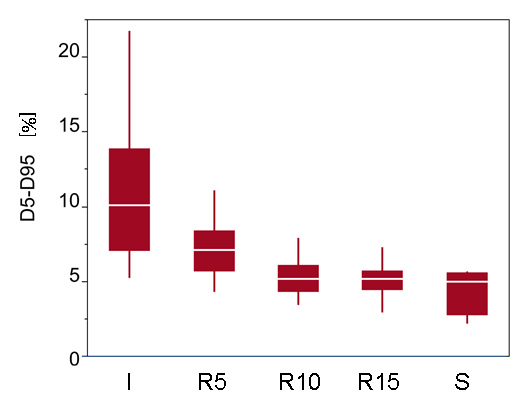
\includegraphics[scale=0.35]{./teile/results_porcine/D5D95_Korr_MMT.png}
 }
 \subfigure[V95]{
 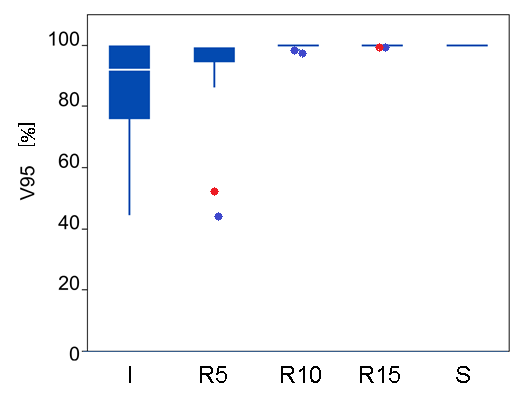
\includegraphics[scale=0.35]{./teile/results_porcine/V95_Korr_MMT_2.png}
 }
  \subfigure[V107]{
 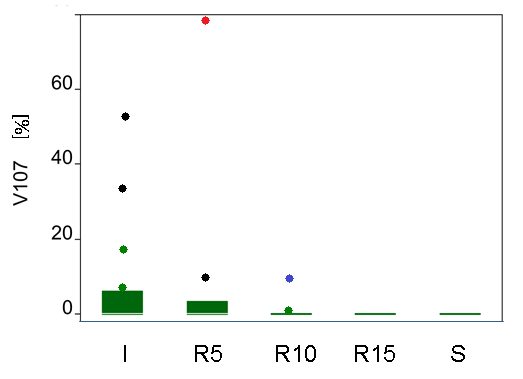
\includegraphics[scale=0.375]{./teile/results_porcine/V107_Korr_MMT_2.png}
}
\caption{Boxplot of dose analysis parameters D5-D95, V95 and V107 over all porcine data sets (pig 1: black, pig 2: blue, pig 3: red, pig 4: green) 
and motion patterns depending on the used technique (I: interplay, R5: five rescans, R10: ten rescans, R15: fifteen rescans, S: static). 
Figures are courtesy of Dr. Christian Graeff.}
\label{static_interplay_rescanning_ALLpigs_KORR}
\end{figure}

% \vspace*{-0.4cm}

Figure \ref{static_interplay_rescanning_ALLpigs_KORR} shows the results of the dose analysis parameters over all pigs and motion patterns 
depending on the studied technique. It can be seen that for all studied cases, rescanning yields improved dose depositions compared to the 
interplay case. For D5-D95 the median of the ideal, static case is 5.0\% (75th percentile: 5.6\%), which 
increases to 10.1\% (13.9\%) for the interplay distribution. With five rescans this can be already be improved to 7.1\% (8.4\%). A slightly 
better improvement is observed from ten rescans on, whereas no further benefit result from more than ten rescans (5.2\% (6.1\%) for ten rescans 
versus 5.2\% (5.7\%) for fifteen rescans). As this dose analysis parameter was normally distributed, the correlation between the dose homogeneity 
and rescan number was analyzed. Thereby interplay was included as a rescan number of one. 
The proportion of variance explained resulted in $r^{2}$=0.46 (p<0.0001). 
For V95 interplay resulted to have a median of 92.1\% (25th percentile: 75.9\%) versus 100\% (100\%) for the static case. The dose coverage 
could be improved to 99.8\% (25th percentile: 94.5\%) with five rescans and even to 100\% (100\%) for ten and fifteen rescans. 
For the over dosage the static case was found to have a median of 0\% (75th percentile: 0\%) which increased to 0\% (6.3\%) for interplay and 
could be reduced to 0\% (0\%) already with five rescans.\newline
\newline
It can be concluded that five rescans are already sufficient to improve the interplay results, but ten or more rescans are needed in order 
to have treatment planning results comparable to the static irradiation. 
In order to enable a correct dose-escalation study ten rescans are hence favorable. For the here studied motion pattern and porcine data 
set cases this rescan number would lead to a dose deposition corresponding to the planned dose deposition. 

\newpage

\subsubsection{Irradiation time}

In figure \ref{irrTime_rescan15} the irradiation time for rescanning of AV node are shown for all pigs and the two studied 
beam channel directions (couch angle 90$^{\circ}$ and -90$^{\circ}$). 
The stated results were achieved with a low intensity irradiation (minimal particle number of 75,000 per beam spot)\footnote{as this resulted 
in the maximal particle number still yielding a homogenous dose deposition in case of static irradiation. Further analysis is needed}. 
For an irradiation with 5mm margin 
the treatment time over all pig data sets results to a mean value of about one minute per field (see table \ref{tab:rescan_time:pigs}). 
Thus the overall treatment time would result to (1.9 $\pm$ 0.1)min with rescanning as motion mitigation technique for heartbeat motion 
in porcine data. Theoretically, this result could be further reduced with a higher minimum particle number and hence a higher irradiation 
intensity. Nevertheless these irradiation times are already very short due to the small target volume. It needs to be observed in 
the upcoming experiments if these short treatment times can be verified. 

\vspace*{0.5cm}

 \begin{figure}[H]
 \begin{center}
 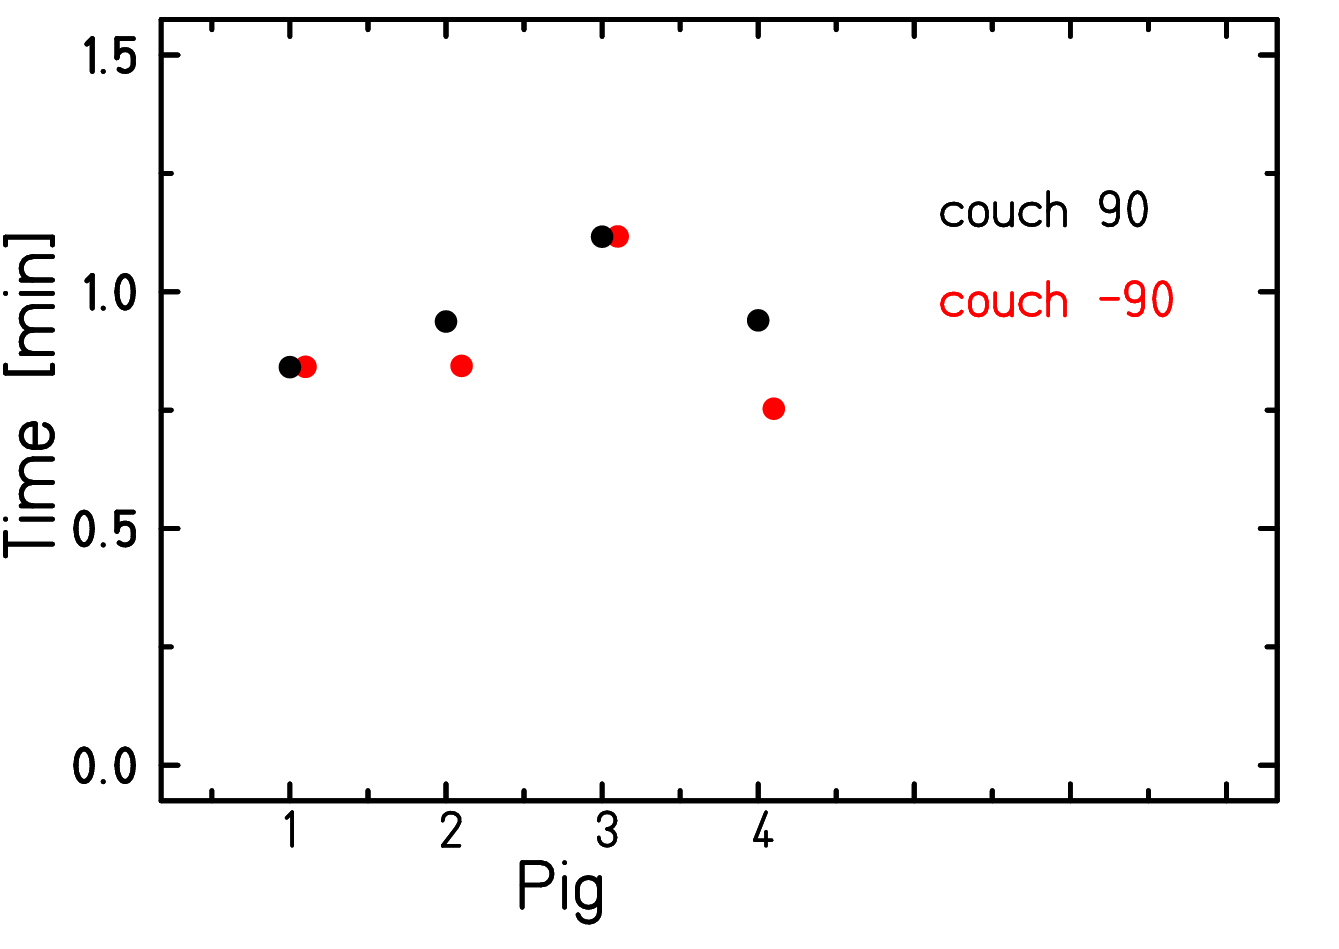
\includegraphics[scale=0.2]{./teile/results_porcine/Rescan15_irrTime.png}
\caption{Irradiation time of fifteen rescans for all pigs and beam entry channels.}
\label{irrTime_rescan15}
 \end{center}
\end{figure}

\begin{table}[H]
  \centering
  \caption{Mean irradiation time for AV node with a safety margin of 5mm over all pigs.}
  \begin{tabular}{|c|c|}
    \hline\hline
    Couch angle [$^{\circ}$] & time [min] \\
    \hline
    -90 & 0.9 $\pm$ 0.1 \\
    90 & 1.0 $\pm$ 0.1 \\ \hline
    total & 1.9 $\pm$ 0.1 \\
    \hline\hline
    \end{tabular}
  \label{tab:rescan_time:pigs}
\end{table}


\newpage

\section{Discussion}
\label{pigs:diss}
In this chapter the influence of heartbeat motion on different cardiac target volumes (PVs, CTI, AV node) in porcine data sets was studied 
and treatment planning studies with rescanning as motion mitigation technique were carried out. The dose deposition to OAR, including 
cardiac substructures, was analyzed. This analysis is motivated by the planned experiments on the feasibility of the non-invasive ablation of 
cardiac target sites with carbon ions in pigs. In experimental cardiology, dogs as well as pigs are most frequently used. As dogs are known to 
display certain differences in anatomy and physiology compared to man \cite{Hug86, Cri98} it is planned to use pigs in the upcoming GSI 
experiments.\newline
\newline
Even though it seems to be accepted in literature that the anatomy of pig hearts are very similar to that of humans 
\cite{Lum66, Dou72, Hug86, Coo91, Whi93} Crick et al. \cite{Cri98} carried out a detailed comparison between the 
anatomy of porcine and human hearts. They found several significant differences which they suspected to arise mainly from the different 
orientation of the bodys (unguligrade versus orthograde) and hence location of the heart in the thorax and from the differing form of 
the thorax itself. While the upper and lower borders of the hearts were found to have similar size and features, the general shape differs as 
the pig hearts are more 'Valentine' shaped and the human hearts more trapezoidal. This also leads to important differences in the internal 
anatomy. While in human hearts the right atrium is typically larger than the left, the atria of pigs have a similar size. Concerning the left 
atrium, only two orifices for the pulmonary veins exist, while humans have four pulmonary vein openings. The right atrium was furthermore 
stated to differ significantly from the human heart, especially in the atrial appendage. 
Regarding the ventricles Crick et al. stated that the right ventricle was observed to have a similar structure like human hearts, such as 
the tricuspid and pulmonary valvar arrangements. But also here differences were found (e.g. the orientation of the pulmonary valve). 
The left ventricles seem to have similar features to the human structure, but the ventricular wall was found to be much thicker in porcine. 
Furthermore it was stated that the left chambers of the pig hearts were significantly bigger compared to the right chambers, so that the 
apex was found to be composed entirely of left ventricular musculature. Also in human hearts the left ventricle is bigger than the right one. 
Concerning coronary circulation it was noted that most pigs displayed a blood supply to the sinus and atrioventricular node by branches 
of the right coronary artery, while in humans this is observed to a lesser extent.\newline
\newline
Due to the different anatomy of pigs compared to humans it was expected to find different results in the motion of the cardiac target volumes 
as well as in the dose deposition to the OAR. The findings will be discussed in the next subsections. 

\subsection{Movement of cardiac target volumes in cardiac cycle}

Due to the dense muscular structure of the heart contrast enhanced CT scans were acquired in comparison to native scans. Deformable image 
registrations were carried out on both data sets and the resulting motion displacement of the cardiac target volumes were assessed. It 
could be concluded that native CT scans do not enable an estimation of either the motion amplitude or direction. While e.g. the mean absolute displacement 
of the AV node was found to (0.1 $\pm$ 0.1)mm in the native scans of pig 3, the mean absolute displacement on contrast CT scans was found to 
be (2.0 $\pm$ 0.4)mm. This difference is sufficient to completely alter the results of the treatment planning study as
an interplay pattern would be expected with the motion field from the contrast enhanced CT scans, while the motion of the native scans would 
be too small to yield an interplay effect. 
It is thus obvious that contrast enhanced CT scans are needed in order to correctly assess the motion of the cardiac target volumes. 
As contrast enhanced CT scans change the Hounsfield unit information, which are needed for range informations in particle therapy, it is 
not intented to deliver treatment plans created on these data sets. In the case of treatment planning studies for pure feasibility  
it can nevertheless be accepted as the range information does not need to be applied. In the planned experiments at GSI a strategy to use 
the motion displacement field of the contrast enhanced CT, while carrying out the treatment planning on native CT scans, is nevertheless needed. 
A first concept could be to enable a robust stabilization of the pigs during CT acquisition so that no position difference between the native 
CT scan and the injection of the contrast agent is induced. This would hence enable a direct application of the 
deformation field of the contrast enhanced CTs on the native CT scans.\newline
\newline
Based on the contrast enhanced CT scans the motion of the cardiac target volumes - PV, CTI and AV node - in all four porcine 
data sets was assessed. It could be observed that the CTI moved the most in all four pigs, followed by the AV node. The PV moved to a lesser 
extend in all four pigs. It was assumed that these findings were connected to the location of the target volumes within the heart, where 
the PVs are found in the upper atria and the CTI in the lower atria, hence increasing the influence of the stronger ventricular motion. 
As the AV node is found in between ventricles and atria it can be hypothesized that the position is more stable and hence the influence 
of the ventricular motion on the displacement of the structure is slightly reduced. Furthermore it was found that in all four  
porcine data sets as well as for all three studied cardiac target volumes the displacement in AP direction was larger than in the other two 
motion directions (SI and LR). For the porcine data sets a shallower motion range of the target 
volumes was furthermore observed in-between MP 6 and 13, enabling a potential application of gating as another motion mitigation technique 
for the compensation of heartbeat motion in swines. Nevertheless a close analysis of the individual motion pattern of the respective pig 
is needed as the motion differed among the animals. 


\subsection{Dose to organs at risk for the irradiation of AV node}

Due to a lack of corresponding data dose-volume limits for the studied OAR (esophagus, trachea, aorta and heart) were taken from the RTOG 
protocols for SBRT treatments of humans. These limits were not exceeded in the irradiation of AV node with 5mm safety margin. 
It can be argued that this is due to the large distance of the target volume from the analyzed critical structures. Nevertheless the resulting 
dose deposition with carbon ions is also smaller than the results for photon irradiation. A study by radiologists from the collaborating 
Mayo Clinic \cite{Song14} stated that an IMRT irradiation of the AV node with 5-6mm margin and (32 $\pm$ 0.6)Gy in the same porcine data sets 
resulted in a mean dose to the esophagus of 1.6Gy. In case of carbon ions no dose deposition was found in this structure (mean: (0 $\pm$ 0)Gy). 
The mean dose to the trachea was found to be 2.2Gy with IMRT delivery, while also here no dose was deposited with carbon ions (mean: (0 $\pm$ 0)Gy). 
Concerning the mean overall cardiac dose it was stated that an IMRT delivery would result in (4.7 $\pm$ 1.3)Gy. For carbon ions a mean 
cardiac dose of (0.03 $\pm$ 0.00)\% of the physical dose was found, resulting in (0.7 $\pm$ 0.1)Gy for 25Gy or (1.0 $\pm$ 0.1)Gy for 32Gy, respectively. 
The better sparing of the critical structures with carbon ions compared to IMRT is on one hand due to the reduced beam channel number. 
On the other hand the physical advantages of carbon ions compared to photon delivery (e.g. Bragg peak) become obvious in these results. 
For a more detailed comparison of OAR dose depositions with photons compared to carbon ions, the reader shall be referred to chapter 
\ref{Discussion}, section \ref{Dose:OAR:photons}. 
The study by Song et al. also included an analysis of the dose deposition when irradiating the AV node with proton beams \cite{Song14}. Here a 
single AP field was applied, resulting in (30.7 $\pm$ 0.2)Gy to the AV node. The mean overall cardiac dose was stated to result to (3.6 $\pm$ 1.5) Gy. 
The dose deposition to the surrounding heart is hence higher in case of proton irradiation compared to carbon ions. This is especially striking 
since only one field was used in proton treatment compared to the here presented two carbon ion beam channels, hence resulting in a bigger 
irradiated cardiac volume. Nevertheless it should be kept in mind that the beam channels can not be directly compared, since two lateral 
fields were used in carbon ion treatment planning, while a single AP field was applied in proton therapy.\newline
\newline
The dose deposition in the cardiac substructures was also studied in the AV node irradiations with carbon ions. The LV resulted 
to receive a slighthy higher maximum point dose compared to the RV, while the mean dose in the two structures were comparable and the 
maximal irradiated volume was smaller for the LV compared to the RV. In the study by Crick et. al it is stated that the LV is significantly 
bigger compared to the RV in swines and that sensitive structures like the apex are composed entirely of LV musculature \cite{Cri98}. It can 
thus be understood why the maximal irradiated volume of the LV is significantly smaller than the RV even though the beam channels are 
symmetrical in lateral position. Concerning the coronary arteries it was found that the mean and maximal point dose to the LCA is smaller than 
the RCA and also the maximal irradiated volume of the LCA is smaller compared to the RCA. Since no dose limit information exist it is unclear 
whether the larger exposure of the RCA compared to LCA is problematic, especially since pigs were found to supply the SA and AV node via branches of the RCA.


\vspace*{-0.3cm}
\subsection{Rescanning as motion mitigation technique for AV node irradiation}

In the irradiation of cardiac volumes in the animal study carried out at CyberHeart and at Universit\"atsklinikum 
Schleswig-Holstein in L\"ubeck, both with photons, only an ITV approach was used in order to compensate for heartbeat motion \cite{Sha10, Bla13}. 
Due to the interference effects between the active carbon ion beam application and the assessed motion of up to 6mm of the AV node due to heartbeat, 
a different approach was needed for carbon ions. Rescanning was studied as potential motion mitigation technique for the non-invasive 
ablation of the AV node with an underlying heartbeat motion in swines.\newline
\newline
By analyzing the dose coverage, dose homogeneity and over dosage for different underlying motion patterns it was found that rescanning results 
in an appliable dose deposition. The dose coverage was higher than 99\% in 85\% of all studied cases 
and even increased to 91\% of the studied cases when more than ten rescans were analyzed (100\% for only fifteen rescans). V107 values 
higher than 0\% were obtained in 15\% of all cases, which further reduced to 6\% of the studied cases when only the DVHs for ten and fifteen 
rescans were evaluated. V107=0\% was found in all studied cases for fifteen rescans. The dose homogeneity D5-D95 did not exceed 8\% for ten 
rescans. This value could be slightly improved to 7\% with fifteen rescans. For five rescans, the dose homogeneity reached up to 11\%.
It could be concluded that rescanning with ten rescans yields better results compared to only five rescans, while 
additional rescans do lead to a further improvement of the outcome.\newline
\newline
All these results were found for slice-by-slice rescanning, which means that each IES is irradiated independently with the predefined number 
of rescans and the adapted particle numbers. In this case the treatment time is not prolonged. It needs to be studied if other rescanning 
techniques like breath-sampled rescanning \cite{Sec09} or phase-controlled rescanning \cite{Fur07}, where the rescanning of the individual IES 
are sampled according to the motion phase of the breathing period, are applicable to cardiac motion (ECG-sampled rescanning). Due to the 
shallower displacement of the porcine cardiac target volumes between motion phase six and thirteen, gating \cite{Kub96} on the cardiac cycle 
might be another feasible motion mitigation technique. In order to keep the treatment time as short as possible a fast beam extraction 
modality for synchrotrons with radiofrequency knock-out exciters is needed. This exist, e.g., at the National Institute of Radiological 
Science (NIRS) in Japan \cite{Nod96, Fur05} and at the Heidelberg Ion Therapy Center (HIT) \cite{Schoe11}. 


\vspace*{-0.3cm}
\section{Conclusion}

Contrast enhanced CT scans are needed in order to assess the motion of cardiac target volumes due to heartbeat motion. 
Potential cardiac target volumes in swine move due to heartbeat with an amplitude of up to a couple of millimeters and the 
dominant motion direction was found to be in AP direction. The displacement of the AV node creates interplay effects when 
irradiated with carbon ions. Rescanning as motion mitigation technique was studied. 
Rescanning with fifteen rescans yields improved dose analysis parameters compared to interplay in all studied pig cases and for all 
underlying motion patterns and achieved results comparable to the static irradiations. It is thus an adequate motion mitigation technique for 
the planned experimental validation in animal models where the AV node will be irradiated. Dose-volume limits to the surrounding OAR were not 
exceeded. 



